%\section{Espacios vectoriales con producto interno}
%\chapter{Espacios vectoriales con producto interno}
\chapter{Espacios vectoriales con prod. int.}
Los conceptos geométricos de longitud, distancia y perpendicularidad, que son bien conocidos para   $\mathbb{R}^2$ y $\mathbb{R}^3$, se definen en este capítulo  para cualquier espacio vectorial euclídeo $V$. Estos conceptos  proporcionan herramientas geométricas potentes para resolver muchos problemas aplicados, incluidos los problemas de mínimos cuadrados. Los tres conceptos se definen en términos del  producto escalar o  producto interior, de dos vectores.

\section{Producto interno. Ejemplos}\index{Producto interno}


\bigskip

\begin{definition} \index{Producto interno}
\label{Prod.int.}
\bigskip

Sea $V$ un espacio vectorial sobre $\mathbb{R}$ o $\mathbb{C}$. Un \textit{producto interno} sobre $V$ es una función $\phi :  V \times V\rightarrow \mathbb{R}$ (o $\mathbb{C}$) que cumple:

\bigskip


\begin{enumerate}

\item   $\phi(\vec{x},\vec{y})=\overline{\phi(\vec{y},\vec{x})} $  para todo $\vec{x}$, $ \vec{y}$ $\in V$

\bigskip


\item  

$\phi(\vec{x}+\vec{z},\vec{y}   )=\phi(\vec{x},\vec{y}) + \phi(\vec{z},\vec{y})$, para todos  $ \vec{x}$, $ ~\vec{y}$, $ ~\vec{z} $ $\in V$

\bigskip


\item $\phi(\alpha\vec{x},\vec{y})=\alpha\phi(\vec{x},\vec{y})$ para todo $\vec{x}$,$\vec{y}$ $\in V$ y todo $\alpha \in \mathbb{R} $ o $\mathbb{C}$

\bigskip

\item  $\phi(\vec{x},\vec{x})> 0$ para todo $\vec{x}\neq 0$

\end{enumerate}
\end{definition}

\bigskip


\bigskip


\begin{remark}
\label{ObsPI}


Consecuencias de $1$, $2$ y $3$:

\begin{itemize}
    
\item 

De $1.$  y $2.$ se deduce 

\bigskip



$\phi(\vec{x},\vec{y}+\vec{z}   )=\phi(\vec{x},\vec{y}) + \phi(\vec{x},\vec{z})$, para todos $ \vec{x}$, $ ~\vec{y}$, $ ~\vec{z} $ $\in V$.

\bigskip

\item 

De $3.$ y de $1.$ se deduce que 

\bigskip


$\phi(\vec{x},\alpha \vec{y})=\overline {\alpha }\phi(\vec{x},\vec{y})$ para todo $\vec{x}$, $\vec{y}$ $\in V$ y todo $\alpha \in \mathbb{R}$.



\bigskip

\item 

De $2.$ se deduce que 

\bigskip


$\phi(\vec{0}+\vec{y},\vec{x}   )=\phi(\vec{y},\vec{x}) = \phi(\vec{0},\vec{x})+ \phi(\vec{y},\vec{x})$, sí y sólo sí $\phi(\vec{0},\vec{x})=0$. 


\bigskip

Por la propiedad simétrica $\phi(\vec{x},\vec{0})=0$  y, en particular, $\phi(\vec{x},\vec{x})=0$ si $\vec{x}=\vec{0}$.




\end{itemize}
%\hfill$\blacktriangle$
\end{remark}


\bigskip

\begin{example}

\newpage

Los productos internos  en $\mathbb{R}^n$  y $\mathbb{C}^n$ son,   respectivamente:
  
\bigskip

$$ \phi(\vec{x},\vec{y})= \phi((x_1, x_2, \cdots, x_n),  (y_1, y_2, \cdots, y_n))= x_1y_1+ x_2 y_2+ \cdots + x_ny_n   \qquad (\mathbb{R}^n) $$

 $$ \phi(\vec{x},\vec{y})= \phi((x_1, x_2, \cdots, x_n),  (y_1, y_2, \cdots, y_n))= x_1 \overline y_1+ x_2 \overline y_2+ \cdots + x_n\overline y_n  \qquad (\mathbb{C}^n)$$
 
\bigskip

Son los productos internos  canónicos.
Se deja al lector la verificación de las propiedades $1-4$ de la Definición \ref{Prod.int.} en cada caso.
\end{example}


\bigskip

\begin{remark}
\label{ObsPII}
\begin{itemize}
    \item 
A un espacio vectorial real  (o complejo) $V$ provisto de un producto interno se lo llama espacio  \textit{Espacio euclídeo}, $\mathbb{E}$, (respectivamente, \textit{unitario}). 
    \item

El producto interno generaliza el producto escalar de los vectores $\Vec{x}$ e $\Vec{y}$ $ \in \mathbb{R}^n$ a un espacio vectorial $V$ cualquiera.
    \item 
Si se tiene un producto interno, se anotará   $\phi(\vec{x},\vec{y})=(\vec{x},\vec{y})$
\end{itemize}
\end{remark}


\bigskip





\begin{example}
\label{PRODINTL2}
En el espacio vectorial de las funciones continuas en $[a,b]$, $C([a,b])$, a valores reales,  se define

$$\phi :  C([a,b]) \times C([a,b]) \rightarrow \mathbb{R}$$

$$ \phi(f,g)=  \int_a^b  f(t) g(t) dt.$$

\bigskip

En el caso de funciones a valores complejos,  se define $ \phi(f,g)=  \int_a^b  f(t) \overline g(t) dt$  (similar a $\mathbb{C}^2$).

\end{example}
\begin{remark}
\begin{itemize}
    \item
El producto interno anterior es el que se utiliza para hallar los coeficientes de la serie de Fourier de una función $f(x)$  en $[0, 2 \pi]$.  Se calculan con el producto interno entre la función $f(x)$ y la base ortogonal $ \{e^{inx}\}_{n \in Z}$ o $\{1, cos(nx), sen(nx)\}_{n \in N}$.
\item
La serie de Fourier tiene importantes aplicaciones, por ejemplo, en el procesamiento de señales. Permite la descomposición de la señal en una base ortonormal y obtener sus componentes frecuenciales. En señales de música posibilita  separar los instrumentos.
\end{itemize}
%\hfill$\blacktriangle$
\end{remark}


\bigskip

Una vez fijada una base de $V$,   si $V$ es un espacio vectorial de dimensión finita con un producto interno,  es posible construir una matriz asociada al producto interno y a dicha base.




\section{Matriz de un producto Interno.}\index{Matriz de un producto interno}

%\textbf{DEFINICIÓN: Matriz de un producto interno} 

\bigskip

Sea $V$ un espacio vectorial sobre $\mathbb{R}$ o $\mathbb{C}$ de dimensión finita con producto interno y sea $B= \left\{\vec{v}_1,\vec{v}_2,\cdots, \vec{v}_n\right\}$ una base de $V$. Se define  la \textit{matriz del producto interno}  $(\cdot,\cdot)$  en la base $B$ como la matriz  $\in \mathbb{R }^{n \times n }$  (resp. $\in \mathbb{C }^{n \times n }$)  tal que $$P_ {ij}= (\vec{v}_i,\vec{v}_j)  \quad1\leq i,j\leq n$$



Esta matriz nos permite calcular el producto interno entre cualquier par de vectores. Si $\vec{x}=\sum^{n}_{i=1}x_i \vec{v}_i~$  e $~\vec{y}=\sum^{n}_{j=1}y_j \vec{v}_j$

\bigskip




$$(\vec{x},\vec{y})=(\sum^{n}_{i=1}x_i \vec{v}_i,\sum^{n}_{j=1}y_j \vec{v}_j)= \sum^{n}_{i=1}\sum^{n}_{j=1}x_i \overline {y}_j ~(\vec{v}_i,\vec{v}_j) $$

\bigskip

\noindent
En particular, para $n=3$, se tiene

$$(\vec{x},\vec{y})=(x_1, x_2, x_3) \left(\begin{array}{ccc}  (\vec{v}_1, \vec{v}_1)  & (\vec{v}_1, \vec{v}_2)  & (\vec{v}_1, \vec{v}_3)   \\ (\vec{v}_2, \vec{v}_1) & (\vec{v}_2, \vec{v}_2)  & (\vec{v}_2, \vec{v}_3)  \\ (\vec{v}_3 , \vec{v}_1 )  & (\vec{v}_3 , \vec{v}_2 )& (\vec{v}_3, \vec{v}_3 )\end{array}
 \right) \left(\begin{array}{c} \overline y_{1} \\ \overline y_{2}  
\\  \overline y_3 
\end{array}\right)$$

\bigskip

\bigskip


\begin{remark}
    Si $P$ es la matriz de un producto interno, entonces $P_{ij}=\overline P_{ji}$  para todo $i\neq j$. Sin embargo, esa condición no es suficiente para que $P$ sea la matriz de un producto interno. Por ejemplo, la matriz  

$$A= \left(\begin{array}{cc}  0 & 1  \\ 1 &  1
\end{array}
 \right)$$
 
 \bigskip
 
 \noindent
 no puede ser la matriz de un producto interno en una base, ya que si $ \vec v$ es el primer vector de la base, se tendría $(\vec v,\vec v)=0$ y sería el vector nulo.
\end{remark}

 



%\textbf{Ejemplos:}



\section{Longitud, ángulos, distancia y ortogonalidad.}

\bigskip

A partir de la definición de un producto interno, es posible  generalizar las nociones de longitud, ángulos, distancia y ortogonalidad ya vistas para vectores de $\mathbb{R}^{2}$ y $\mathbb{R}^{3}$.

\bigskip

\begin{definition}\index{Longitud de un vector}
\textbf{Longitud o norma de un vector} $\vec{x}$ en un espacio  con producto interno se define como
\begin{equation}
 \left\| \vec{x}\right\|=\sqrt{(\vec{x},\vec{x})},\qquad \vec{x}\in \mathbb{E} 
 \label{10}
\end{equation}
\end{definition}

\bigskip

\begin{example}
En $\mathbb{R}^2 $, si $\vec{v}= (a , b)$,  $\left\| \vec{v}\right\| $  es la longitud del segmento que va desde el origen hasta $\vec{v}$, y es consecuencia del Teorema de Pitágoras (ver Figura \ref{PITAGORAS}).




\end{example}
\index{Longitud de un vector}

\bigskip

\begin{example}
\label{EX1chap6}
 Sea $\vec{x}=(1,-2,2,0)$. Como $\left\| \vec{x}\right\|^2=(1)^2+(-2)^2+(2)^2=9$,
su longitud o norma euclídea  es $\left\| \vec{x}\right\|=\sqrt{9}=3.$   
\end{example}

\bigskip


\begin{remark}
    \begin{itemize}
\item

La definición de longitud   tiene sentido por la propiedad $4.$ del producto interno (Definición  \ref{Prod.int.}).


\item

Se tiene  la propiedad siguiente:

$$\left\|\alpha \vec{x}\right\|= \sqrt{(\alpha\vec{x},\alpha\vec{x})}=\sqrt{\alpha^{2}(\vec{x},\vec{x})}=\left|\alpha\right|\sqrt{(\vec{x},\vec{x})}=\left|\alpha\right|\left\|\vec{x}\right\|$$


\item
Todo vector de longitud $1$ se dice \textit{unitario}; todo vector $\vec{x}$ no nulo de un espacio euclídeo puede \textit{normalizarse}, es decir, hacerlo unitario multiplicándolo por $\frac {1}{\left\|\vec{x}\right\|}$.
%\[
%\frac {1}{\left\|\vec{x}\right\|}.
%\]
\end{itemize}
%\hfill$\blacktriangle$
\end{remark}





\begin{figure}
    \centering
    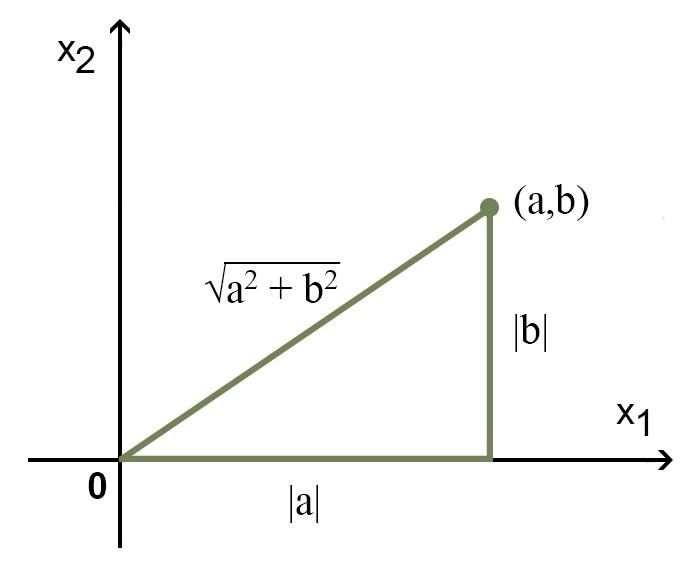
\includegraphics[width=0.50\textwidth]{Pictures/PITAGORAS.jpg}
    \caption{La norma da la longitud del vector.}
    \label{PITAGORAS}
\end{figure}

\bigskip

\begin{example}
    

El vector unitario $\vec{u} \in \mathbb{R}^4$ que tiene la misma dirección que el vector $\vec{x}$ del Ejemplo \ref{EX1chap6} es



\begin{equation}
\vec{u}=\frac{\vec{x}}{\left\| \vec{x} \right\|}=(\frac{1}{3}, -\frac{2}{3}, \frac{2}{3},0)
 \label{20}
\end{equation}
\end{example}  

\bigskip



%Ver para $\mathbb{R}^{2}$ primero Lay pag 381 y hacer gráfico

\textbf{Ángulo entre dos vectores.}\index{Angulo entre dos vectores.}


\bigskip

En $\mathbb{R}^{2}$ el producto escalar verifica la expresión que sigue:
\begin{equation}
 (\vec{x},\vec{y})   = \left\|\vec{x}\right\|\left\|\vec{y}\right\|cos \theta
 \label{30}
\end{equation}


La verificación para $\mathbb{R}^{3}$ es similar. Cuando $n > 3$, puede usarse la Ec.(\ref{30})  para
definir el ángulo entre dos vectores de $\mathbb{R}^{n}$, o en espacios vectoriales cualesquiera. 


\bigskip

Dados dos vectores $\vec{x}$ e $\vec{y}$ de un espacio euclídeo, definimos el \textit{coseno} del ángulo  entre ellos como 

\begin{equation}
cos (\theta)=\frac {(\vec{x},\vec{y})} {\left\|\vec{x}\right\|\left\|\vec{y}\right\|} 
  \label{444}
  \end{equation}


\bigskip

Para que tenga sentido la definición anterior, es necesario demostrar que el valor absoluto del cociente
\[\frac {(\vec{x},\vec{y})} {\left\|\vec{x}\right\|\left\|\vec{y}\right\|}\] 

\bigskip
\noindent
sea menor que o igual que $1$.

\bigskip
\begin{remark}
En Estadística, el valor de $cos (\theta)$ definido mediante la Ec.(\ref{444}) para los vectores $\vec{x}$ e $\vec{y}$ es llamado  \textit{coeficiente de correlación entre los vectores $\vec{x}$ e $\vec{y}$}, y mide de alguna forma la similitud entre ambos.
%\hfill$\blacktriangle$
\end{remark}

\bigskip

\index{Cauchy, Augustin Louis}
\begin{parchment}[ Augustin Louis Cauchy (1789-1857)]{Fue un matemático francés, miembro de la Academia de Ciencias de Francia y profesor en la Escuela politécnica.
Cauchy ha sido uno de los matemáticos más prolíficos de todos los tiempos, solo superado por Leonhard Euler, Paul Erdős y Arthur Cayley con cerca de 800 publicaciones y siete trabajos; su investigación cubre el conjunto de áreas matemáticas de la época. Fue pionero en análisis donde se le debe la introducción de las funciones holomorfas, los criterios de convergencia de series y las series de potencias. Sus trabajos sobre permutaciones fueron precursores de la teoría de grupos, contribuyendo de manera medular a su desarrollo. En óptica se le atribuyen trabajos sobre la propagación de ondas electromagnéticas. \cite{Cauchy}}
\end{parchment}
%{ Nació en París y murió en una villa cercana a esa misma ciudad. Fue autor de trabajos importantes sobre ecuaciones %diferenciales, series infinitas, determinantes, probabilidad, grupos de permutación y de física matemática. En 1814 %publicó una memoria que se convirtió en el fundamento de la teoría de las funciones complejas. Su trabajo se conoce %por su rigor. Publicó 789 artículos y ocupó puestos en la Facultad de Ciencias, en el Colegio de Francia y en la %Escuela Politécnica, todos en París. Existen muchos términos y teoremas que llevan su apellido. Fue un realista fiel y %vivió en Suiza, Turín y Praga. Regresó a París en 1838 y recuperó su puesto en la Academia de Ciencias. En 1848 %recuperó su lugar en la Sorbona, que mantuvo hasta su muerte.}



\bigskip

\begin{theorem}\textbf{Desigualdad de Cauchy-Schwartz:}\index{Desigualdad de Cauchy-Schwartz}
\label{PROPOSICIÓN 6.39:}



En todo espacio vectorial con producto interno, 

$$\left|{(\vec{x},\vec{y})}\right|\leq {\left\|\vec{x}\right\|\left\|\vec{y}\right\|}$$
\noindent
para todo  $\vec{x}$,$~\vec{y}$  $\in \mathbb{E}$.

\bigskip

\begin{proof}

Si $\vec{y}=\vec{0}$ vale, pues $\left|{(\vec{x},\vec{0})}\right|=0 \leq \left\|\vec{x}\right
\|0=0$.

\bigskip

Si $\vec{y}\neq \vec{0}$,

\bigskip

\[0 \leq (\vec{x}-\frac {(\vec{x},\vec{y})\vec{y}} {\left\|\vec{y}\right\|^2},\vec{x}-\frac {(\vec{x},\vec{y})\vec{y}} {\left\|\vec{y}\right\|^2})
\]
\bigskip

\[
0 \leq (\vec{x},\vec{x}-\frac {(\vec{x},\vec{y})\vec{y}} {\left\|\vec{y}\right\|^2})-\frac {(\vec{x},\vec{y})} {\left\|\vec{y}\right\|^2} (\vec{y},\vec{x}-\frac {(\vec{x},\vec{y})\vec{y}} {\left\|\vec{y}\right\|^2})
\]

\bigskip

\[0 \leq (\vec{x},\vec{x})- \overline{(\vec{x},\vec{y}}+\frac {(\vec{x},\vec{y})} {\left\|\vec{y}\right\|^2}  - \frac {(\vec{x},\vec{y})} {\left\|\vec{y}\right\|^2}(\vec{y},\vec{x}) + \frac {(\vec{x},\vec{y})} {\left\|\vec{y}\right\|^2}\frac {\overline{(\vec{x},\vec{y})}} {\left\|\vec{y}\right\|^2}(\vec{y},\vec{y})
\]

\bigskip


\[0 \leq (\vec{x},\vec{x})- \overline{(\vec{x},\vec{y})}\frac {(\vec{x},\vec{y})} {\left\|\vec{y}\right\|^2}  - \frac {(\vec{x},\vec{y})} {\left\|\vec{y}\right\|^2}(\vec{y},\vec{x}) + \frac {(\vec{x},\vec{y})} {\left\|\vec{y}\right\|^2}\frac {{(\vec{y},\vec{x})}} {\left\|\vec{y}\right\|^2}(\vec{y},\vec{y})
\]

\bigskip


Como $\left\|\vec{y}\right\|^2=(\vec{y},\vec{y})$, se cancelan los dos últimos términos. Entonces,

\bigskip

\[0 \leq \left\|\vec{x}\right\|^2 - \frac {\left|{(\vec{x},\vec{y})}\right|^2} {\left\|\vec{y}\right\|^2}
\]
\noindent
que equivale a 

\[0 \leq  \frac {\left\|\vec{x}\right\|^2 \left\|\vec{y}\right\|^2 -\left|{(\vec{x},\vec{y})}\right|^2} {\left\|\vec{y}\right\|^2}
\]
\bigskip

En el numerador se tiene la desigualdad que se quería demostrar.

\end{proof}
\end{theorem}







\begin{remark}
Se acredita a Cauchy la desigualdad para vectores y a Schwarz para los productos escalares con integrales. Sin embargo, fue Bunyakovsky quien demostró y publicó la desigualdad de Schwarz en una monografía, 25 años antes que Schwarz.
%\hfill$\blacktriangle$   
\end{remark}

\bigskip







\section{Distancia entre vectores.}

\bigskip

\begin{definition}\index{Distancia entre vectores}
%\textbf{Distancia entre vectores}



Sea $V$ un espacio vectorial sobre $\mathbb{R}$ o $\mathbb{C}$ con producto interno. Se define la distancia $d$, $d :  V \times V\rightarrow \mathbb{R}$  como:

$$d(\vec{x},\vec{y})=\left\|\vec{x}-\vec{y}\right\|.$$
\end{definition}

\bigskip

Usando las propiedades de la norma, se puede verificar que $d$ satisface:

\bigskip

\begin{enumerate}

\item   $d(\vec{x},\vec{y}) \geq 0 $  para todo $\vec{x}$,$~\vec{y}$ $\in E$

\bigskip

\item   $d(\vec{x},\vec{y})= 0 $  sí y sólo sí  $\vec{x}=\vec{y}$ 

\bigskip

\item   $d(\vec{x},\vec{y})= d(\vec{y},\vec{x})$  para todo $\vec{x}$,$~\vec{y}$ $\in E$

\bigskip

 \item  $d(\vec{x},\vec{z})\leq d(\vec{x},\vec{y})+ d(\vec{y},\vec{z})   $  para todo $\vec{x}$, $~\vec{y}$, $~\vec{z}$ $\in E$.

\bigskip

\bigskip

\bigskip

\end{enumerate}

\index{Schwarz, Karl  Herman  }
\begin{parchment}[Karl Herman Amandus Schwarz (1843-1921)] {Fue un matemático alemán conocido por su trabajo en análisis complejo. Schwarz inicialmente estudio química en Berlín pero Kummer y Weierstrass lo persuadieron para que se hiciera matemático. Entre 1867 y 1869 trabajó en Halle, después en Zürich. Desde 1875 trabajó en el universidad de Gotinga, tratando los temas de teoría de funciones, geometría diferencial y cálculo de variaciones. Su memoria en ocasión del 70 aniversario de Weierstrass contiene, entre otros temas importantes, la desigualdad para integrales que hoy se conoce como desigualdad de Schwarz. \cite{schwarz} }
\end{parchment}




\bigskip




\index{Bunyakovsky, Viktor Yakovlevich}
\begin{parchment}[Viktor Yakovlevich Bunyakovsky (1804-1889)]{ Nació en Ucrania. Estudió matemáticas en la Sorbona, en la que se doctoró en 1825 bajo la tutoría de Augustin Cauchy.1​
En 1826 volvió a San Petersburgo donde ejerció como profesor de la Escuela de Cadetes de la Academia Naval y del Instituto de Comunicaciones. De 1846 a 1880 fue profesor en la Universidad de San Petersburgo. 

Entre otros campos de las matemáticas, Buniakovski trabajó sobre todo en teoría de números, análisis matemático y en teoría de la probabilidad. Son relevantes las aportaciones que llevan su nombre como la conjetura de Buniakovski (nunca demostrada) y la desigualdad de Cauchy-Buniakovski-Schwarz. Sus aportaciones más originales son en teoría de la probabilidad, acerca de la cual publicó numerosos artículos sobre el estudio de problemas estadísticos de la población de Rusia. \cite{buny}   } 
\end{parchment}


\bigskip

\bigskip






\begin{figure}
    \centering
    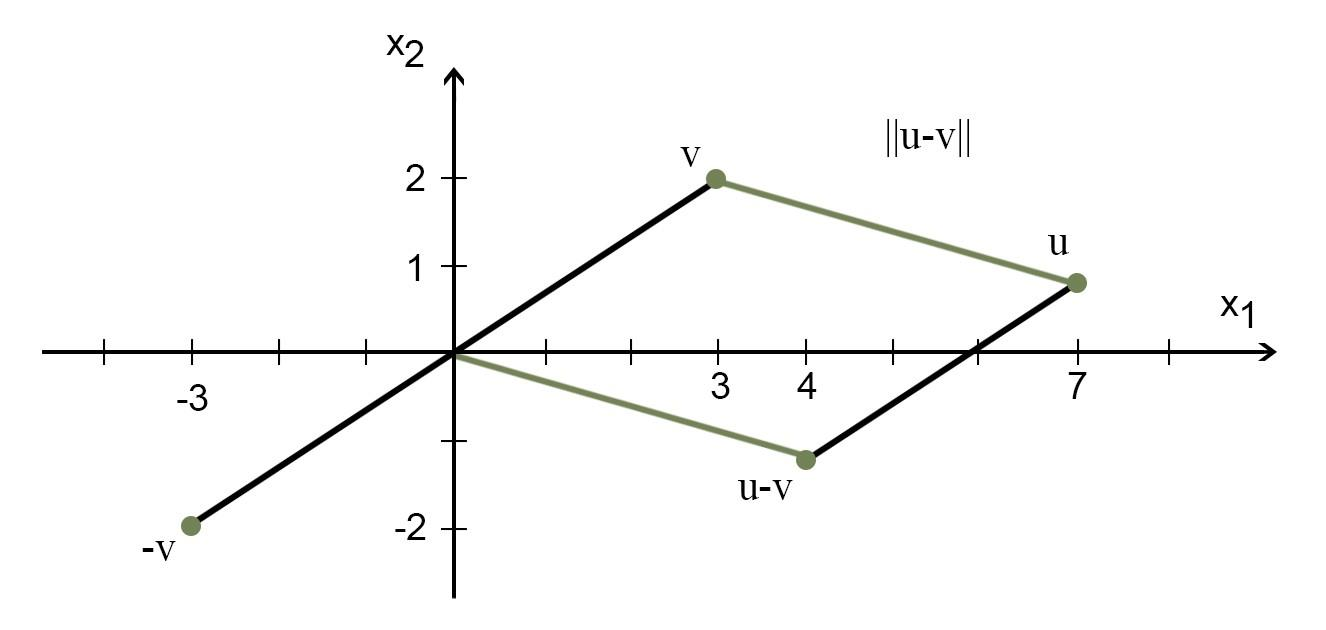
\includegraphics[width=0.80\textwidth]{Pictures/DISTANCIA.jpg}
    \caption{Distancia entre los vectores $\vec{u}$ y $\vec{v}$. }
    \label{DISTANCIA}
\end{figure}

\bigskip

\begin{example}
    

En la Figura \ref{DISTANCIA} se muestran los vectores $\vec{u}$, $\vec{v}$ y $\vec{u}- \vec{v}$,

$$ \vec{u}- \vec{v}= \left(\begin{array}{c}  7  \\ 1
\end{array}
 \right)-   \left(\begin{array}{c}  3  \\ 2 
\end{array}
 \right) =   \left(\begin{array}{c}  4  \\ -1
\end{array}
 \right)$$ 

$$\left\|\vec{u}-\vec{v}\right\|= \sqrt{ 4^4+ (-1)^2}=\sqrt{17}.$$

Puede observarse que la distancia de $\vec{v}$ a $\vec{u}$ es la misma que la de $\vec{u}- \vec{v}$ a $\vec{0}$, y también que si se suma el vector $\vec{u}- \vec{v}$ a $\vec{v}$ se obtiene el vector $\vec{u}$.
\end{example} 

\begin{remark}
\begin{itemize}
    \item 

     Dados dos vectores   $\vec{x}$ e $\vec{y}$, se dice que $d(\vec{x},\vec{y})$ es la \textit{distancia} entre $\vec{x}$ e $\vec{y}$.
     \item 

     Una distancia es una función  que verifica las $4$ propiedades anteriores. Puede no provenir de ninguna norma.
\end{itemize}
 %\hfill$\blacktriangle$   
\end{remark}






\bigskip

Con la definición que sigue se  generaliza  la noción de perpendicularidad entre vectores de un espacio vectorial. 

\bigskip
\begin{definition}

Sea $V$ un espacio vectorial sobre $\mathbb{R}$ o $\mathbb{C}$ con producto interno. Dos vectores $\vec{x}$, $\vec{y}$ se dicen \textit{ortogonales} (o perpendiculares), si
\begin{equation}
(\vec{x},\vec{y})=0
\label{40}
\end{equation}

\end{definition}

\bigskip

\begin{remark}
Por las propiedades vistas en las  observaciones \textcolor{blue}{{\fontfamily{qcr}\selectfont{i}}} en la Sección \ref{ObsPI}, el vector nulo,  es ortogonal a todo vector de $V$.
%\hfill$\blacktriangle$   
\end{remark}




\begin{corollary}
    
\textbf{Teorema de Pitágoras} 
\label{Pitagoras}


Dos vectores $\vec{x}$ e $\vec{y}$  son ortogonales, sii 

$$\left\|\vec{x}+\vec{y}\right\|^{2}=\left\|\vec{x}\right\|^{2}+\left\|\vec{y}\right\|^{2}$$

\end{corollary}

\bigskip

La demostración se deja al lector.


\bigskip


\begin{definition} 

Sea $V$ un espacio vectorial sobre $\mathbb{R}$ o $\mathbb{C}$ de dimensión finita con producto interno. Se dice que $\left\{\vec{v}_1,\vec{v}_2,\cdots, \vec{v}_r\right\}\subset V$ es un conjunto ortogonal si $(\vec{v}_i,\vec{v}_j)=0$ para todo $i\neq j$. \end{definition}

\bigskip

\begin{example}
 \label{eju1u2u3}   

El conjunto  $S=\{\vec{u_1}, \vec{u_2}, \vec{u_3}\}$, 
donde $\vec{u_1}=(3,1,1)^T$, $\vec{u_2}=(-1,2,1)^T$ y $\vec{u_3}=(-1/2,-2,7/2)^T$,
es un conjunto ortogonal, ya que al considerar los tres pares posibles de vectores, 

\bigskip

$\{\vec{u_1}, \vec{u_2}\}$, $\{\vec{u_1},\vec{u_3}\}$, y $\{\vec{u_2}, \vec{u_3}\}$, se tiene 

 \bigskip 

$\vec{u}_1 \cdot \vec{u}_2= 3(−1) + 1(2) + 1(1)= 0$

\bigskip

$\vec{u}_1 \cdot \vec{u}_3= 3(−1/2) + 1(-2) + 1(7/2)= 0$

\bigskip

$\vec{u}_2 \cdot \vec{u}_3= -1(−1/2) + 2(-2) + 1(7/2)= 0$

\bigskip



Cada par de vectores distintos es ortogonal, así que $S=\{\vec{u_1}, \vec{u_2}, \vec{u_3}\}$, es un conjunto ortogonal como se muestra  en  la Figura \ref{Conj.Ortog}. 
\end{example}



\begin{figure}
    \centering
    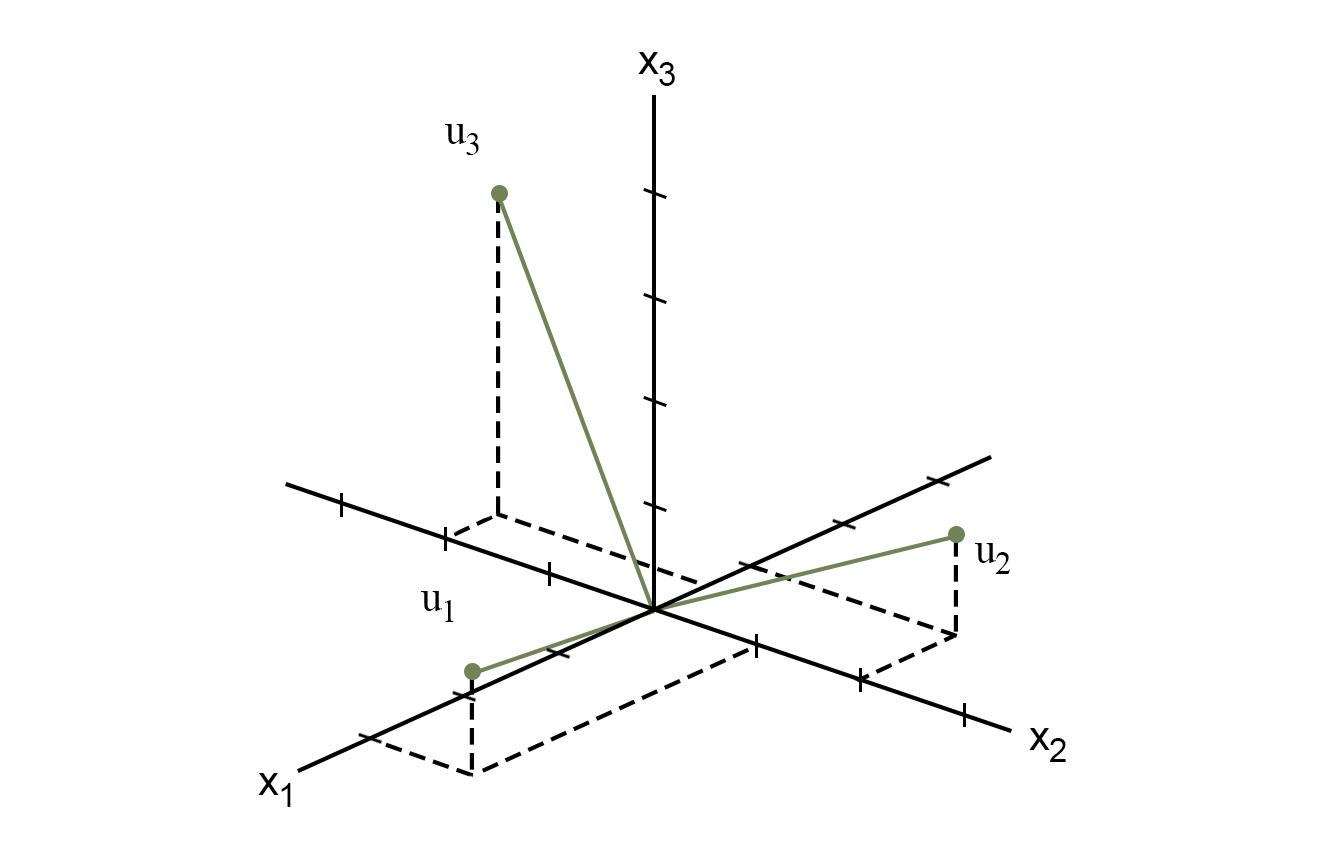
\includegraphics[width=0.80\textwidth]{Pictures/fig.28.jpg}
    \caption{$\{\vec{u_1}, \vec{u_2}, \vec{u_3}\}$ es un conjunto ortogonal de $\mathbb{R}^3$.}
    \label{Conj.Ortog}
\end{figure}

\bigskip

\begin{remark}
Un conjunto de $r$ vectores se dice \textit{ortonormal} si es ortogonal y $\left\|\vec{u}_i\right\|=1$  para cada $1\leq i\leq r$.
%\hfill$\blacktriangle$  
\end{remark}

\bigskip

\begin{theorem}

Sea $V$ un espacio vectorial sobre $\mathbb{R}$ o $\mathbb{C}$ de dimensión finita con producto interno y sea $\left\{\vec{v}_1,\vec{v}_2,\cdots, \vec{v}_r\right\}\subset V$  un conjunto ortogo-\ nal de $V$ con $\vec{v}_i\neq \vec{0}$  para  $1\leq i\leq r$. Entonces  $\left\{\vec{v}_1,\vec{v}_2,\cdots, \vec{v}_r\right\}$ es un conjunto de vectores  linealmente independiente.

\begin{proof}

Supongamos que $\sum_{i=1}^r  \alpha_i \vec{v}_i = \vec{0}$. Entonces, para cada $j$, $ 1 \leq j \leq r$,


$$ 0=(\vec{0}, \vec{v}_j)= ( \sum_{i=1}^r  \alpha_i \vec{v}_i,\vec{v}_j) = \sum_{i=1}^r  \alpha_i (\vec{v}_i,\vec{v}_j )= \alpha_j \left\|\vec{v}_j\right\|^{2}, $$

\noindent
y como $\vec{v}_j \neq \vec{0}$,  $ \alpha_j=0$ para  $ 1 \leq j \leq r$ y entonces, $\left\{\vec{v}_1,\vec{v}_2,\cdots, \vec{v}_r\right\}$ es un conjunto de vectores linealmente independiente.

 
\end{proof}

\end{theorem}

\bigskip

En el teorema siguiente se muestra por qué una base ortogonal es mucho mejor que otras bases: las coordenadas de un vector en esa base  pueden calcularse muy  fácilmente.

\bigskip


\begin{theorem}

Sea $V$ un espacio vectorial sobre $\mathbb{R}$ o $\mathbb{C}$ de dimensión finita con producto interno y sea $\left\{\vec{v}_1,\vec{v}_2,\cdots, \vec{v}_r\right\}\subset V$ es un conjunto ortogonal de $V$ con $\vec{v}_i\neq \vec{0}$  para  $1\leq i\leq r$. Sea $\vec{v} \in \left\langle \vec{v}_1,\vec{v}_2,\cdots, \vec{v}_r\right\rangle$. Entonces 


\begin{equation}
  \vec{v} =\sum^{r}_{j=1}   \frac {(\vec{v}, \vec{v}_j)} {\left\|\vec{v}_j\right\|^{2}} \vec{v}_j
  \label{50}
\end{equation}


\begin{proof}
 Si  $ \vec{v} = \sum_{i=1}^r  \alpha_i \vec{v}_i$, para cada $j$, $ 1 \leq j \leq r$, se tiene que 

 $$ (\vec{v}, \vec{v}_j)= ( \sum_{i=1}^r  \alpha_i \vec{v}_i,\vec{v}_j) = \sum_{i=1}^r  \alpha_i (\vec{v}_i,\vec{v}_j )= \alpha_j (\vec{v}_i,\vec{v}_j ) =\alpha_j \left\|\vec{v}_j\right\|^{2}, $$

\noindent 
 y como $\vec{v}_j\neq \vec{0}$, se tiene entonces que \[\alpha_j = \frac{(\vec{v}, \vec{v}_j)}{\left\|\vec{v}_j\right\|^{2}}\]
\end{proof}

\end{theorem}

\bigskip


\begin{example}
\label{EJ48}
El conjunto $\{\vec{u_1}, \vec{u_2}, \vec{u_3}\}$  del Ejemplo \ref{eju1u2u3}   es una base ortogonal para
$\mathbb{R}^3$. Si se  desea expresar el vector $\vec{y}=(6,1,-8)^T$ como una combinación lineal de los vectores en $S$,
de acuerdo a la  Ec.(\ref{50}) se tiene que, 

\begin{equation*}
  \vec{y} =\sum^{3}_{j=1}   \frac {(\vec{y}, \vec{u}_j)} {\left\|\vec{u}_j\right\|^{2}} \vec{u}_j
  \label{60}
\end{equation*}

\bigskip

Para hallar las coordenadas de $\vec{y}$ en la base ortogonal,   se  calculan los productos escalares

\bigskip

$\vec{y}. \vec{u_1}= 11$, $\vec{y}. \vec{u_2}= -12$, $\vec{y}. \vec{u_3}= -33$

\bigskip
y 
$\vec{u_1}. \vec{u_1}= 11$, $\vec{u_2}. \vec{u_2}= 6$, $\vec{u_3}. \vec{u_3}= 33/2$



 \bigskip

\begin{equation*}
  \frac {(\vec{y}, \vec{u}_1)} {\left\|\vec{u}_1\right\|^{2}} \vec{u}_1=\frac{11}{11}(3,1,1) =(3,1,1)
  \label{70}
\end{equation*}

\begin{equation*}
  \frac {(\vec{y}, \vec{u}_2)} {\left\|\vec{u}_2\right\|^{2}} \vec{u}_2=\frac{-12}{6}(-1,2,1)=2(-1,2,1)
  \label{70}
\end{equation*}

\begin{equation*}
   \frac {(\vec{y}, \vec{u}_3)} {\left\|\vec{u}_3\right\|^{2}} \vec{u}_3=\frac{-33}{33/2}(-1/2,-2,7/2)=2(-1/2,-2,7/2)
  \label{80}
\end{equation*}

Y se obtiene, 
\[
\vec{y}= 1 \vec{u}_1 -2 \vec{u}_2 -2 \vec{u}_3 
\]
\noindent
que puede verificarse fácilmente,

$\vec{y}=(6,1,-8)=(3,1,1) -2(-1,2,1) -2 (-1/2,-2,7/2)$.
\end{example}

\bigskip

\begin{remark}
 \begin{itemize}
     \item

     Como se vio en el Ejemplo  \ref{EJ48}, es muy  fácil  calcular las coordenadas de un vector $\vec{y}$ en una base ortogonal. En otro caso,  se debe que resolver un sistema de ecuaciones lineales para hallarlas.
\item
Si el conjunto además, es ortonormal, se tiene

$$ \vec{v} =\sum^{r}_{j=1}   (\vec{v}, \vec{v}_j)  \vec{v}_j $$
 \end{itemize}
 %\hfill$\blacktriangle$
\end{remark}

\bigskip

\bigskip

La proposición que sigue asegura que en todo espacio vectorial de dimensión finita con producto interno tiene  bases ortonormales. Más aún, en la demostración se da un procedimiento recursivo conocido como Gram-Schmidt que permite obtener una base ortonormal del espacio vectorial a partir de una base cualquiera del mismo.


\bigskip

\begin{theorem}
\textbf{ Método de ortonormalización de Gram-Schmidt} \index{Método  de Gram-Schmidt} 

\bigskip

Sea $V$ un espacio vectorial sobre $\mathbb{R}$ o $\mathbb{C}$ de dimensión finita con producto interno y sea $\left\{\vec{v}_1,\vec{v}_2,\cdots, \vec{v}_n\right\}$ una base de $V$. Existe una base ortonormal $B= \left\{\vec{w}_1,\vec{w}_2,\cdots, \vec{w}_n\right\}$ de $V$ tal que 

$$\left\langle \vec{v}_1,\vec{v}_2,\cdots, \vec{v}_k \right\rangle  = \left\langle \vec{w}_1,\vec{w}_2,\cdots, \vec{w}_k \right\rangle $$
para todo $1\leq k \leq n$

%La base ortonormal se obtiene normalizando los vectores de $B$ (dividiendo cada vector de $B$ por su %longitud).


\begin{proof}

Se construyen los vectores  $\left\{\vec{z}_1,\vec{z}_2,\cdots, \vec{z}_n\right\}$ de una base ortogonal, recursivamente



\begin{enumerate}

\item Se toma $\vec{z}_1=\vec{v}_1$  

\bigskip

\item  Se busca $\vec{z}_2 \in V$ tal que $(\vec{z}_2, \vec{z}_1)=0$ y tal que 
$\left\langle \vec{z}_1,\vec{z}_2\right\rangle=\left\langle \vec{v}_1,\vec{v}_2\right\rangle$




\end{enumerate}

\bigskip


La segunda condición vale sí y sólo sí $~\vec{z}_2=a\vec{v}_1+b\vec{v}_2$ con $b\neq 0$. Es  posible considerar $b=1$ y buscar $a$ para que se cumpla la primera condición:

\bigskip



$0=(\vec{z}_2, \vec{z}_1)=(a\vec{v}_1+b\vec{v}_2, \vec{z}_1)= a(\vec{v}_1,\vec{v}_1)+(\vec{v}_2,\vec{v}_1)$,

\noindent 
lo que implica 



$$ a=  \frac {-(\vec{v}_2, \vec{v}_1)} {\left\|\vec{v}_1\right\|^{2}}. $$



Luego, el vector, 

$$ \vec{z}_2= \vec{v}_2 - \frac {(\vec{v}_2, \vec{v}_1)} {\left\|\vec{v}_1\right\|^{2}} \vec{v}_1= \vec{v}_2 - \frac {(\vec{v}_2, \vec{v}_1)} {\left\|\vec{v}_1\right\|^{2}} \vec{z}_1$$
\noindent
satisface las condiciones.

\bigskip


Supongamos construídos $\vec{z}_1, \vec{z}_2,   \cdots, \vec{z}_r \in V$  tales que 

\bigskip

\begin{enumerate}

\bigskip

\item $(\vec z_i,\vec z_j)=0$  cuando $i\neq j$

\bigskip

\item   $\left\langle \vec z_1,\vec z_2, \cdots, \vec z_r \right\rangle=\left\langle \vec v_1,\vec v_2, \cdots, \vec v_r\right\rangle$   con $1\leq k \leq r$


\end{enumerate}
\bigskip

\noindent
consideramos el vector

$$ \vec{z}_{r+1}= \vec{v}_{r+1} -\sum^{r}_{i=1} \frac {(\vec{v}_{r+1}, \vec{z}_i)} {\left\|\vec{z}_i\right\|^{2}} \vec{z}_i$$


\bigskip

Se tiene que 


\bigskip

\begin{itemize}

\item 
$\left\langle \vec{z}_1,\vec{z}_2, \cdots, \vec{z}_r, \vec{z}_{r+1} \right\rangle=\left\langle \vec{v}_1,\vec{v}_2, \cdots, \vec{v}_r,\vec{v}_{r+1}\right\rangle$   con $1\leq k \leq r$

\bigskip

\item  para cada $j\leq r$,  reemplazando $\vec{z}_{r+1}$ y teniendo en cuenta $1.$, 

$$(\vec{z}_{r+1}, \vec{z}_j)=( \vec{v}_{r+1} -\sum^{r}_{i=1} \frac {(\vec{v}_{r+1}, \vec{z}_i)} {\left\|\vec{z}_i\right\|^{2}} \vec{z}_i, \vec{z}_j)$$


$$(\vec{z}_{r+1}, \vec{z}_j)=( \vec{v}_{r+1},, \vec{z}_j) - \frac {(\vec{v}_{r+1}, \vec{z}_j)} {\left\|\vec{z}_j\right\|^{2}}( \vec{z}_j, \vec{z}_j)=0$$


\end{itemize}

\bigskip

Luego $\vec{z}_{r+1}$ satisface las condiciones requeridas.

\bigskip

De esta manera, al concluir el $n$-ésimo paso, se obtiene una base ortogonal $\left\{\vec{z}_1,\vec{z}_2,\cdots, \vec{z}_n\right\}$ de $V$ que además satisface

$$\left\langle \vec{v}_1,\vec{v}_2,\cdots, \vec{v}_k \right\rangle  = \left\langle \vec{z}_1,\vec{z}_2,\cdots, \vec{z}_k \right\rangle $$
para todo $1\leq k \leq n$.

\bigskip

Finalmente, para cada $1\leq i \leq n$ consideramos el vector   $\vec{w}_i=\frac {\vec{z}_i} {\left\|\vec{z}_i \right\|}$. Luego, el conjunto $B= \left\{\vec{w}_1,\vec{w}_2,\cdots, \vec{w}_n\right\}$ resulta una base de $V$ que cumple lo pedido.

\end{proof}
\end{theorem}



\bigskip


\bigskip


\textcolor{blue}{\textbf{Corolario}}
Sea $V$ un espacio vectorial sobre $\mathbb{R}$ o $\mathbb{C}$ de dimensión finita con producto interno y sea $S$ un subespacio   de $V$, $S\neq \{\vec{0}\}$. Entonces existe una base ortonormal de $V$ que contiene una base ortonormal de $S$.
Se demuestra tomando una base de $S$, completando a una base de $V$ y aplicando a esta base el procedimiento de Gram-Schmidt.
{\hfill{\tiny\ensuremath{\blacksquare}}

\bigskip

\bigskip

%\end{document}



\begin{example} \textbf{Aplicación del  Método de Gram-Schmidt}

\bigskip

Dada la base $B= \left\{(1,0,i),(1,1,2+i),(0,0,1)\right\}$ de $\mathbb{C}^{3}$ se desea hallar una base ortonormal con G-S.

\bigskip

$\vec{v}_1= (1,0,i)  $, $\vec{v}_2= (1,1,2+i)$    y $\vec{v}_3=(0,0,1)$ 

\bigskip






$\vec{z}_{1}= \vec{v}_{1}$



\[
 \vec{z}_{2}= \vec{v}_{2} -\frac {(\vec{v}_2, \vec{z}_1)} {\left\|\vec{z}_1\right\|^{2}} \vec{z}_1 
\]



\[\vec{z}_{2}= (1,1,2+i) -\frac {((1,1,2+i), (1,0,i))} {\left\|(1,0,i)\right\|^{2}} (1,0,i)
\]


\[\vec{z}_{2}= (1,1,2+i) -(1-i) (1,0,i)=(i,1,1)
\]


y luego, 




\[ \vec{z}_{3}= \vec{v}_{3} - \frac {(\vec{v}_{3}, \vec{z}_1)} {\left\|\vec{z}_1\right\|^{2}} \vec{z}_1 - \frac {(\vec{v}_{3}, \vec{z}_2)} {\left\|\vec{z}_2\right\|^{2}} \vec{z}_2 
\]
\bigskip


$ \vec{z}_{3}=(i/6,-1/3,1/6)$

\bigskip

$\left\{\vec{z}_1,\vec{z}_2, \vec{z}_3\right\}$ resulta una base de ortogonal de $\mathbb{C}^{3}$ 

\bigskip

Diviendo por su norma queda una base ortonormal $\left\{\vec{w}_1,\vec{w}_2, \vec{w}_3\right\}$

\bigskip

donde $\vec{w}_1=(1/\sqrt{2},0,i/\sqrt{2})$

\bigskip

$\vec{w}_2=(i/\sqrt{3},1/\sqrt{3} , 1/\sqrt{3})$

\bigskip

$\vec{w}_3=(\sqrt{6}i/6,-\sqrt{6}/3 , \sqrt{6}/6)$
  
\end{example}

\bigskip

\bigskip
%\end{document}
La existencia de bases ortogonales para subespacios de dimensión finita de un espacio
con producto interior puede establecerse por medio del proceso Gram-Schmidt, de igual
forma que en $\mathbb{R}^n$. Al aplicar este proceso, es posible plantear ciertas bases ortogonales
que surgen con frecuencia en las aplicaciones y  construir la proyección ortogonal de un vector sobre un subespacio $S$. La proyección no depende de la selección de la
base ortogonal y tiene muy buenas propiedades que se describirán más adelante.
%descritas en el teorema de la descomposición
%ortogonal y en el teorema de la mejor aproximación (ver).
En el teorema que sigue se ve cómo es posible escribir la matriz de una transformación lineal usando producto interno para escribir las coordenadas de la imagen de cada vector de la base ortogonal.

\bigskip

\begin{corollary}
    

Si $T$ es una transformación lineal sobre $V$, $V$ es un espacio vectorial con producto interno y de 
dimensión finita, entonces

$$ (T)_B=((T(\vec{u_j}),\vec{u_i})_{ij}$$
siendo $B=\{\vec{u_1}, \vec{u_2},\cdots  \vec{u_n}\}$ cualquier base ortonormal de $V$.

\begin{proof}
$T(\vec{u}_1)=k_1\vec{u}_1+k_2\vec{u}_2+ \cdots +k_n\vec{u}_n.$

\bigskip

En la primer columna de la matriz deben ir las coordenadas   de $T(\vec{u}_1)$, o sea  $k_1$,  $\cdots  k_n$.

\bigskip
\noindent
y resulta que, las coordenadas son

\bigskip

$(T(\vec{u}_1),\vec{u}_i )= T(k_1\vec{u}_1+k_2\vec{u}_2\cdots+k_n\vec{u}_n,\vec{u}_i)$

\bigskip

$=k_1 (\vec{u}_1,\vec{u}_1) +  k_2 (\vec{u}_1,\vec{u}_2) + \cdots  k_n (\vec{u}_1,\vec{u}_n) = k_i$

\end{proof}
\end{corollary}


\bigskip

\subsection{Complemento Ortogonal}\index{Complemento ortogonal}

\bigskip


\begin{definition}\index{Complemento ortogonal}
    Sea $V$ un espacio vectorial sobre $\mathbb{R}$ o $\mathbb{C}$  con producto interno y sea $S$ un subespacio de $V$. Se define el complemento ortogonal de $S$ como 


\bigskip

$S^{\perp} = \left\{\vec{v}\in V \quad (\vec{v}, \vec{s})=0 \quad \forall \vec{s} ~\in S \right\}$
\end{definition}
\bigskip

\begin{remark}
$S^{\perp}$ es un subespacio de $V$.
\end{remark}  





\begin{example}
Para el subespacio de  $\mathbb{R}^{2}$ generado por el vector $(1,1)$, su complemento ortogonal es  $\left\langle (1,1)\right\rangle^{\perp}=\left\{(x,y) \in \mathbb{R}^{2}, ((x,y),(1,1))=0 \right\}= \left\{(x,y) \in \mathbb{R}^{2}, \quad x+y=0 \right\}=\left\langle (1,-1)\right\rangle$.
\end{example}


\bigskip

\begin{example}
Sea $W$ un plano que pasa por el origen en $\mathbb{R}^3$, y sea $L$ la recta que pasa
por el origen y es perpendicular a $W$. Si $\Vec{u}_1$ y $\Vec{u}_2$ son diferentes de $\Vec{0}$, $\Vec{u}_1$ está sobre $L$, y $\Vec{u}_2$ está en $W$, $\Vec{u}_1 \cdot \Vec{u}_2= 0$, como se muestra en la  Figura \ref{321PROYORTOG}. Así que cada vector sobre $L$ es ortogonal a cada vector $\Vec{w}$ en $W$. De hecho, $L$ consiste en todos los vectores que son ortogonales a los $\Vec{w}$ en
$W$, y $W$ consiste en todos los vectores ortogonales a los vectores  en $L$. Es decir,
$L = W^{\perp}$ y $W = L^{\perp}$. ❚
\end{example} 




\begin{figure}
    \centering
    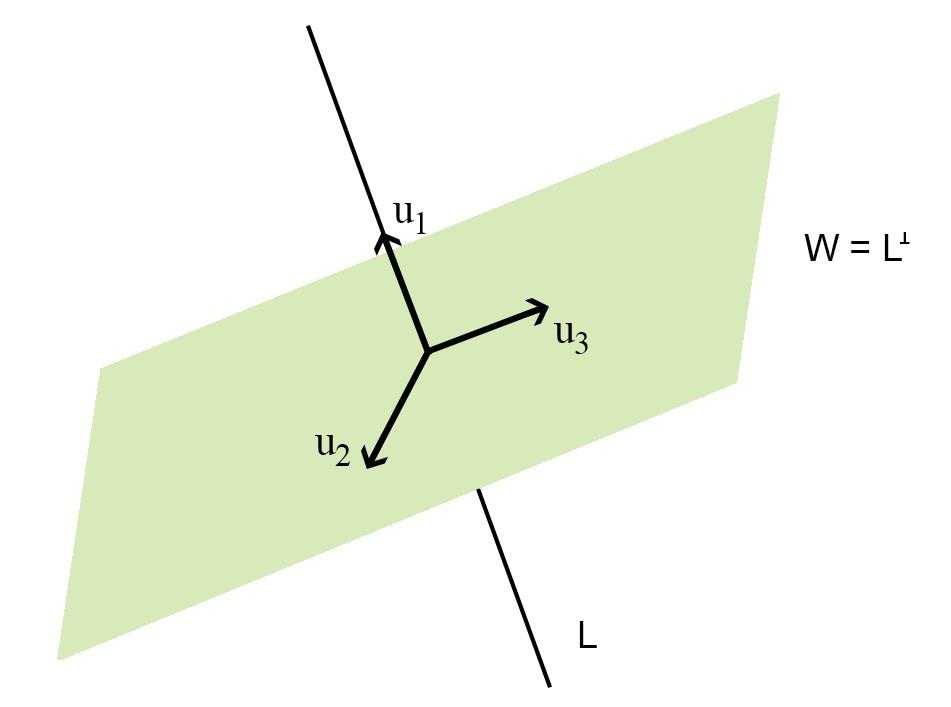
\includegraphics[width=0.80\textwidth]{Pictures/fig.321.jpg}
    \caption{Complemento ortogonal.}
    \label{321PROYORTOG}
\end{figure} 


\bigskip

\begin{example}
%Ejemplo hojita 36
En $\mathbb{C}^3$ hallar el complemento ortogonal de $ \langle( 1,i,1+i) \rangle$.
$ \langle( 1,i,1+i) \rangle^t =$
\begin{eqnarray*}
   = \left \{ (x_1,x_2,x_3) \in \mathbb{C}^3, (x_1,x_2,x_3) \cdot (\alpha , \alpha i, \alpha (1+i))=0 \quad \forall \alpha \in \mathbb{C} \right \} \\
     = \left \{ (x_1,x_2,x_3) \in \mathbb{C}^3, x_1 \overline{\alpha} + x_2 \overline{\alpha i }  + x_3  \overline{\alpha}   (\overline{1+i})=0 \quad \forall \alpha \in \mathbb{C} \right \} 
\end{eqnarray*}
De donde  $$   x_1 \overline{\alpha} - x_2 \overline{\alpha} i + x_3 \overline{\alpha} (1-i)=0$$
o 
 $$    \overline{\alpha}( x_1 - x_2 i + x_3 (1-i))=0.$$
 
 Se tiene, entonces, $x_1= x_2 i - x_3 (1-i)$ y resulta 
\begin{eqnarray*}
    \langle( 1,i,1+i) \rangle^t =  \left \{ (x_2 i - x_3 (1-i), x_2, x_3 )= x_2(i,1,0) + x_3 (i-1,0,1) \right \}
\end{eqnarray*}
\end{example}

\bigskip
\index{Espacio columna de una matriz}
\begin{corollary}
Sea $A$ una matriz de $m \times  n$. El complemento ortogonal del espacio fila de $A$, $Fil A$,  (subespacio de $\mathbb{R}^{n}$ que generan los vectores filas de $A$) es
el espacio nulo de $A$, $Nul(A)$ y el complemento ortogonal del espacio columna de $A$, $Col A$, (subespacio de $\mathbb{R}^{m}$ que generan los vectores columnas de $A$) es el
espacio nulo de la matriz $A^T$. Es decir,



\bigskip

$(Fil A)^{\perp} = Nul(A)$ y $(Col A)^{\perp} = Nul(A^T)$
\end{corollary}



\bigskip

\bigskip

\begin{example}
Dada la matriz


\begin{equation}
A= \left(\begin{array}{ccc} 1  & 0  & 2  \\ 1 & 1 & 4
\end{array}
 \right), \label{333}
\end{equation}
\end{example}

\bigskip
\noindent
se describen los espacios $(Fil A)$, $ Nul(A)$ y $(Col A):


$Nul(A)$ son los vectores de $\mathbb{R}^{3}$ soluciones del sistema homogéneo. Esos vectores son perpendiculares a las filas de la matriz $A$, y pertenecen entonces a subespacio $(Fil A)^{\perp}$.

Si ahora se resuelve el sistema homogéneo con la matriz $A^T$, da el vector nulo de $\mathbb{R}^{2}$.
El subespacio que generan las columnas de $A$, $Col A$ es todo $\mathbb{R}^{2}$, pues  hay en las columnas $2$ vectores linealmente independientes. De ahí que el subespacio ortogonal,  $(Col A)^{\perp} = Nul(A^T)= \vec{0}$.

\bigskip

\bigskip

\begin{theorem}

Sea $V$ un espacio vectorial de dimensión finita con producto interno y sea $S\subseteq V$ un subespacio. Entonces


\bigskip

\begin{enumerate}

\item $S \cap S^{\perp} =\vec{0}$

\bigskip

\item $dim(S) + dim(S^{\perp}) = dim(V)$

\end{enumerate}

\bigskip

En consecuencia, $S \oplus S^{\perp}$.

\bigskip

\begin{proof}

\bigskip
\begin{itemize}
    \item 
  Sea   $\vec{v} \in S \cap S^{\perp}$. Como $\vec{v} \in  S^{\perp}$, $(\vec{v},\vec{s})=0$, $\forall \vec{s}\in S$. En particular para $\vec{s}=\vec{v}$, entonces $(\vec{v},\vec{v})=\left\|\vec{v}\right\|^2=0$, de donde $\vec{v}=\vec{0}$.

  \bigskip
     \item 
   Sea $\left\{\vec{s}_1,\vec{s}_2,\cdots,\vec{s}_r\right\}$ una base de $S$. Existen 
   $\vec{v}_{r+1}, \cdots,\vec{v}_n$ tales que \\ $B=\left \{\vec{s}_1,\vec{s}_2,\cdots,\vec{s}_r,\vec{v}_{r+1}, \cdots,\vec{v}_n \right \}$ es una base de $V$. 
   
   Aplicando Gram-Schmidt se obtiene una base ortonormal  de $V$, 
    $B^\prime=\left\{\vec{w}_1,\vec{w}_2,\cdots,\vec{w}_r,\vec{w}_{r+1}, \cdots\vec{w}_n\right\}$ tal que  $$\left\langle \vec{w}_1,\vec{w}_2,\cdots, \vec{w}_r \right\rangle  = \left\langle \vec{s}_1,\vec{s}_2,\cdots, \vec{s}_r \right\rangle=S.$$
    Sea $j > r$. Veamos que $\vec{w}_j \in S^{\perp}$.
    Dado $\vec{s} \in S$, existen escalares $\alpha_1,\cdots,\alpha_r$, tales que $\vec{s}=\sum_{i=1}^r \alpha_i \vec{w}_i  $, entonces
    
    
    $$(\vec{w}_j, \vec{s})=(\vec{w}_j,\sum_{i=1}^r \alpha_i \vec{w}_i)= \sum_{i=1}^r \overline \alpha_i ( \vec{w}_j, \vec{w}_i) =0.$$
    \noindent
    como la base es ortonormal  y $j > r$, $( \vec{w}_j, \vec{w}_i)=0$  para $1 \le i \le r$.
    De donde, $\vec{w}_j \in S^{\perp}$, y se tiene que, 
    
    $$\left\{\vec{w}_{r+1}, \cdots\vec{w}_n\right\}\in S^{\perp},$$ y, por lo tanto, 
    $$\left\langle \vec{w}_1,\vec{w}_2,\cdots, \vec{w}_r \right\rangle \subseteq S^{\perp},$$ por ser $S^{\perp}$ un subespacio. 
    
     \bigskip
     
    $dim (S^{\perp})   \ge dim (\left\{\vec{w}_{r+1}, \cdots\vec{w}_n\right\})=n-r=n-dim(S)$.
     \bigskip
    Entonces,  $dim (S^{\perp})+ dim(S)   \ge n$.
    
     \bigskip 
    Por otro lado como $S \cap S^{\perp} =\{\vec{0}\}$
    $$dim (S^{\perp})+ dim(S)= dim(S^{\perp}+ S) \le dim(V) = n.$$
    
       Entonces, $dim (S^{\perp})+ dim(S)=dim(V)$
    
\end{itemize}

\end{proof}
\end{theorem}


\bigskip

\begin{remark}
Del teorema sale cómo generar  el subespacio $S^{\perp}$, a partir de la base ortonormal de $V$.  $$S^{\perp}=\left\langle\vec{w}_{r+1}, \cdots\vec{w}_n\right\rangle$$
%\hfill$\blacktriangle$
\end{remark}

\bigskip



\bigskip

\begin{theorem}



Sea $V$ un espacio vectorial de dimensión finita con producto interno y sea $S$ un subespacio de $V$. Entonces $(S^{\perp})^{\perp}=S$

\begin{proof}

Por definición, $(S^{\perp})^{\perp}=\{\vec{v} \in V  / \quad (\vec{v}, \vec{w})=0 \quad \forall ~ \vec{w} \in S^{\perp}  \}$.
Veamos que $S \subseteq (S^{\perp})^{\perp}$. Sea  $ \vec{s} \in S$. Para cada $\vec{w}  \in S^{\perp}$ se tiene que $(\vec{s},\vec{w})= \overline {(\vec{w},\vec{s})}=0$, de donde se deduce que  $ \vec{s} \in (
S^{\perp})^{\perp}$.
\end{proof}
\end{theorem}

\bigskip

\section{Proyección ortogonal}

Dado un subespacio $S$ de un espacio vectorial $V$  de dimensión finita con producto interno . Como  $S \oplus S^{\perp}=V$ se puede considerar el proyector $P_S :  V \rightarrow V$ cuya imagen es $S$ y cuyo núcleo es $S^{\perp}$.


\vskip.5cm

\begin{figure}
    \centering
    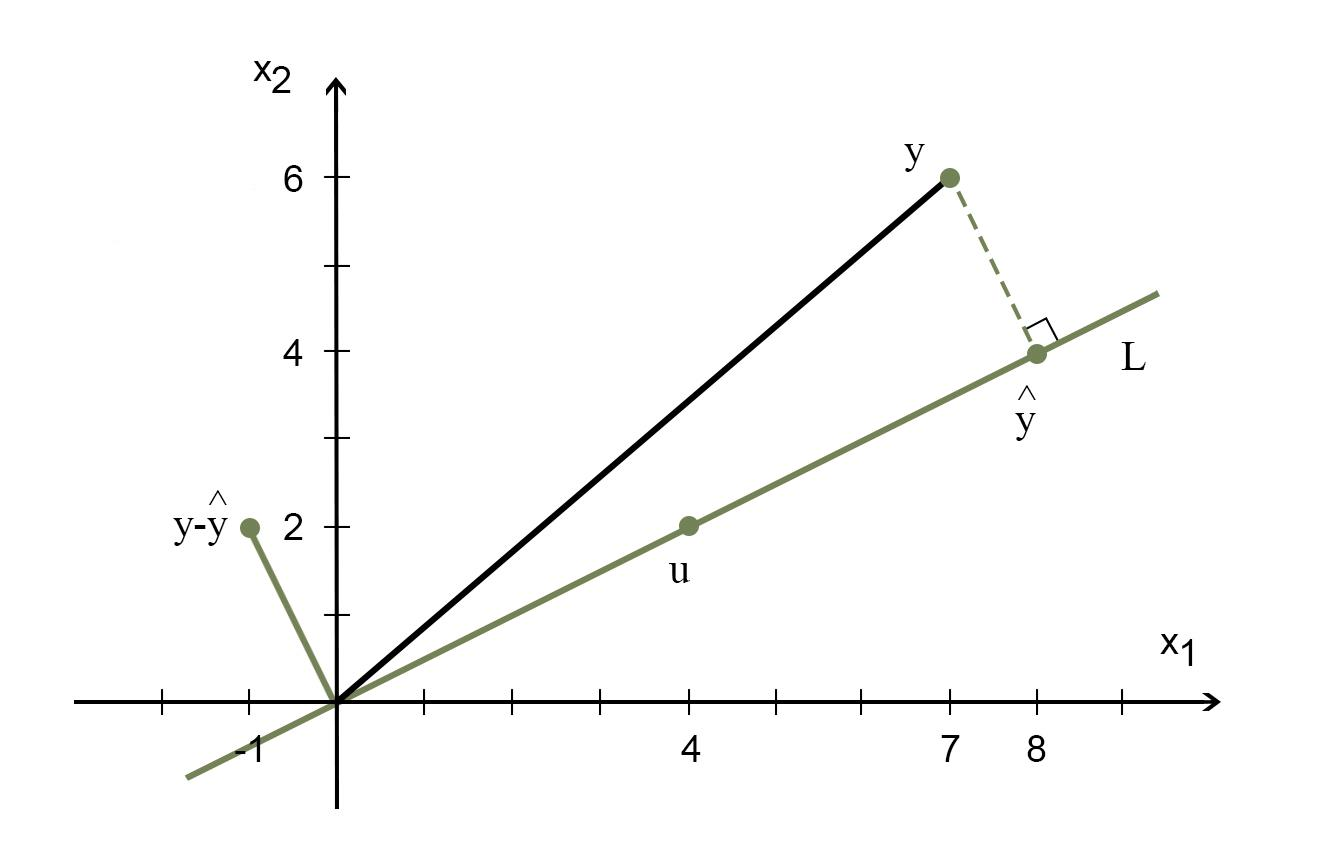
\includegraphics[width=0.80\textwidth]{Pictures/PROYvL.jpg}
    \caption{Proyección del vector $\vec{y}$ sobre la recta $L$. }
    \label{PROYORTOG}
\end{figure}

\begin{definition}
\bigskip
Sea $V$ un espacio vectorial  de dimensión finita con producto interno y sea $S\subseteq V$ un subespacio. Se define la \textit{proyección ortogonal } sobre $S$ como la transformación lineal $P_S :  V \rightarrow V$ que satisface 

\bigskip

\begin{enumerate}

\item $P_S(\vec{s})=\vec{s} $  $ ~ \forall \vec{s}\in S$

\bigskip

\item $P_S(\vec{t})=\vec{0} $  $ ~ \forall \vec{t}\in S^{\perp}$

\end{enumerate}

\end{definition}

\bigskip



\begin{example}
  En $\mathbb{R}^2$  se desea hallar la proyección ortogonal de un vector $\vec{y}$, $ \vec{\hat{y}}$  sobre el subespacio $S$  generado por otro vector $\vec{u} $, o sea sobre la recta $L$ generada por $\vec{u} $ que pasa por el origen. Esto se muestra en la Figura \ref{PROYORTOG}.

  $$P_S(\vec{y})= \vec{\hat{y}}= c \vec{u},$$ y se debe cumplir que $\vec{u} $ sea ortogonal al vector $ \vec{y} -\vec{\hat{y}}$, es decir, $ (\vec{y} -c \vec{u}) \cdot \vec{u}=0 $, entonces,
$$ \vec{y}  \cdot \vec{u} -c \vec{u} \cdot \vec{u}=0  $$
\noindent
  de donde 
  \[c= \frac{\vec{y}  \cdot \vec{u}}{\vec{u} \cdot \vec{u}}
  \]

\noindent
y entonces, la  proyección sobre $L$ es ,
  \begin{equation}
       \label{proyR2}
\vec{\hat{y}}=  \frac{\vec{y}  \cdot \vec{u}}{\vec{u} \cdot \vec{u}}\vec{u}
\end{equation}

  En el caso de la Figura \ref{PROYORTOG}, se tiene que 
  $ \vec{y}= \left(\begin{array}{c}  7  \\ 6
\end{array}
 \right)$  y $\vec{u}=   \left(\begin{array}{c}  4  \\ 2 
\end{array}
 \right).$
 
\bigskip

 Usando Ec.(\ref{proyR2}), como  $\vec{y}  \cdot \vec{u}=40$   y  $\vec{u}  \cdot \vec{u}=20$, se obtiene, 

\bigskip

\[\vec{\hat{y}}=  \frac{\vec{y}  \cdot \vec{u}}{\vec{u} \cdot \vec{u}}\vec{u}= \frac{40}{20}\vec{u}= 2 \vec{u}=\left(\begin{array}{c}  8  \\ 4
\end{array}
 \right)\]
\noindent
 y la componente ortogonal a $  \vec{u}$  es 
 $\vec{y}- \vec{\hat{y}} =\left(\begin{array}{c}  -1  \\ 2
\end{array}
 \right)   .$
 
\bigskip

 La descomposición de $\vec{y}$, como suma de proyecciones sobre $S$ y sobre  $S^{\perp}$, es

 

$$\left(\begin{array}{c}  7  \\ 6
\end{array}
 \right)=\left(\begin{array}{c}  8  \\ 4
\end{array}
 \right)+ \left(\begin{array}{c}  -1  \\ 2
\end{array}
 \right)$$
 
\end{example}

\bigskip

\begin{remark}
\begin{itemize}
    \item 
   Si $B=\left\{\vec{v}_1,\vec{v}_2,\cdots,\vec{v}_r,\vec{v}_{r+1}, \cdots\vec{v}_n\right\}$ una base ortonormal de $V$ tal que $\left\{\vec{v}_1,\vec{v}_2,\cdots,\vec{v}_r\right\}$ es una base de $S$ y $ \left\{\vec{v}_{r+1}, \cdots\vec{v}_n\right\}$ una base de $S^{\perp}$, la proyección ortogonal sobre $S$ es la única transformación lineal $P_S :  V \rightarrow V$ que satisface 

\bigskip

\begin{enumerate}

\item $P_S(\vec{v}_i)=\vec{v}_i $  $ ~ \forall ~ 1 \leq i \leq r$

\bigskip

\item $P_S(\vec{v}_i)=\vec{0} $  $ ~ \forall ~ r+1 \leq i \leq n$

\end{enumerate}

\bigskip

En consecuencia, para $\vec{v}\in V$, recordando que $ \vec{v} =\sum^{n}_{j=1}   (\vec{v}, \vec{v}_j)  \vec{v}_j $   resulta,


%\begin{equation}
% \label{formulaproy}   
%P_S(\vec{v})&= & P_S (\sum^{n}_{j=1}   (\vec{v}, \vec{v}_j)  \vec{v}_j ) \\ 
%P_S(\vec{v})&=& \sum^{n}_{j=1}   (\vec{v}, \vec{v}_j)  P_S (  \vec{v}_j )=\sum^{r}_{j=1}   (\vec{v}, \vec{v}_j)  \vec{v}_j  
%\end{equation}

\begin{equation}
 \label{formulaproy}   
P_S(\vec{v})=  P_S (\sum^{n}_{j=1}   (\vec{v}, \vec{v}_j)  \vec{v}_j )  = \sum^{n}_{j=1}   (\vec{v}, \vec{v}_j)  P_S (  \vec{v}_j )=\sum^{r}_{j=1}   (\vec{v}, \vec{v}_j)  \vec{v}_j,  
\end{equation}



\noindent
que es una expresión para $P_S(\vec{v})$ en términos de los vectores de la base ortonormal de $S$.
 \item
Sea $V$ un espacio vectorial  de dimensión finita con producto interno y sea $S\subseteq V$ un subespacio.
Entonces $P_S+P_{S^{\perp}}=id_V$,

\bigskip
\noindent
donde, 
 $P_S(\vec{v})= \sum^{r}_{j=1}   (\vec{v}, \vec{v}_j)  \vec{v}_j $  y $ ~P_{S^{\perp}}(\vec{v})=\sum^{n}_{j=r+1}   (\vec{v}, \vec{v}_j)  \vec{v}_j.$
    
\end{itemize}
%\hfill$\blacktriangle$
\end{remark}


\bigskip




\begin{example}

\end{example}
Si  $V=\mathbb{R}^4 $ y $W$ es el subespacio 

$$W= \left \{ \vec{x} \in \mathbb{R}^4,~ x_1-2x_2 + x_3= x_1-3x_2 +x_4=0  \right \},$$
se desea hallar la proyección ortogonal del vector $\vec{v}= (4,8,-4,12)$ sobre el subespacio $W$.
	
Para usar la expresión de la Ec.(\ref{formulaproy}) debemos hallar una base ortonormal de $W$.
 En primer lugar calculamos una base de $W$ resolviendo el sistema por eliminación
de Gauss:

\bigskip

\begin{equation}
 \left(\begin{array}{cccc} 1  & -2  & 1 & 0  \\ 1 & -3 & 0 & 1
\end{array}
 \right) \rightarrow  \left(\begin{array}{cccc} 1  & -2  & 1 & 0  \\ 0 & -1 & -1 & 1
\end{array}
 \right)
\end{equation}

\bigskip
A partir de la matriz escalonada, al resolver el sistema homogéneo,  quedan como variables independientes $x_3$ y $x_4$  y una base de $W$ es 

$\left \{ (-3,-1,1,0),(2,1,0,1) \right \}$.  Una base ortogonal,  de $W$ a partir de aplicar Gram-Smichdt  es 
$$  \left \{ (-3,-1,1,0),(\frac{1}{11},\frac{4}{11},\frac{7}{11},1) \right \}. $$ 



Si llamamos $\vec{w}_1=(-3,-1,1,0)$ y $\vec{w}_2=(\frac{1}{11},\frac{4}{11},\frac{7}{11},1)$, los vectores de la base ortonormal $\vec{v}_i$ se obtienen dividiéndolos por su norma, $\vec{v}_i =\frac {\vec{w}_i} {\left\| \vec{w}_i \right\|}.$ 


\bigskip


Entonces,  como $P_W(\vec{v})= \sum^{2}_{j=1}   (\vec{v}, \vec{v}_j)  \vec{v}_j  $, se calculan los productos escalares $(\vec{v}, \vec{v}_j)$, y se obtiene que  

$$P_W((4,8,-4,12))= (\frac{124}{17},\frac{88}{17}, \frac{52}{17}, \frac{140}{17}  )$$


\bigskip

\noindent
es el vector del subespacio  $W$ más cercano a $\vec{v}= (4,8,-4,12)$.


\end{example}

\bigskip

%Es interesante leer el teorema de la mejor aproximación  pag 398 Lay.

\begin{corollary}
    

 Teorema de la proyección ortogonal.
 \label{TPOr}

Sea $S$ un subespacio de un espacio vectorial con producto interno, $V$. Entonces, para cada $\vec{v} \in V$, el vector de $S$ a menor distancia de $\vec{v}$ es $P_S(\vec{v})$.

\begin{proof}



Si $B=\left\{\vec{v}_1,\vec{v}_2,\cdots,\vec{v}_r,\vec{v}_{r+1}, \cdots\vec{v}_n\right\}$ una base ortonormal de $V$ tal que $\left\{\vec{v}_1,\vec{v}_2,\cdots,\vec{v}_r\right\}$ es una base de $S$.

Sea $\vec{v} \in V$. Se tiene que $\vec{v}= \sum^{n}_{j=1}   (\vec{v}, \vec{v}_j)  \vec{v}_j $  y $ ~P_{S}(\vec{v})=\sum^{r}_{j=1}   (\vec{v}, \vec{v}_j)  \vec{v}_j $.
Por otro lado, si $\vec{s} \in S$, $\vec{s}= \sum^{r}_{j=1}   (\vec{s}, \vec{v}_j)  \vec{v}_j  $.


Entonces

$$\vec{v}-\vec{s}= \sum^{n}_{j=1}   (\vec{v}, \vec{v}_j)  \vec{v}_j -  \sum^{r}_{j=1}   (\vec{s}, \vec{v}_j)  \vec{v}_j = \sum^{r}_{j=1}   (\vec{v} - \vec{s}, \vec{v}_j)  \vec{v}_j+ \sum^{n}_{j=r+1}   (\vec{v}, \vec{v}_j)  \vec{v}_j  $$


\noindent
de donde,

$$\left\|\vec{v}-\vec{s}\right\|^2=  \sum^{r}_{j=1}   \left|(\vec{v} - \vec{s}, \vec{v}_j)\right|^2 + \sum^{n}_{j=r+1}  \left| (\vec{v}, \vec{v}_j) \right|^2  \geq    

\sum^{n}_{j=r+1}  \left| (\vec{v}, \vec{v}_j)\right|^2 = \left\|\vec{v}-P_{S}(\vec{v})\right\|^2 $$

\end{proof}

\end{corollary}

\bigskip

\begin{remark}
\begin{itemize}
    \item 
El teorema anterior es conocido también como el Teorema de la mejor aproximación.
\item
En la Figura \ref{PROYORTOG},  $\vec{\hat{y}}$ es el punto de $L$ más cercano a $\vec{y}$, en el sentido que
$$\left\|\vec{y}-\vec{\hat{y}}\right\| \leq \left\|\vec{y}-\vec{v} \right\|,$$
para todo $\vec{v}$ en $L$ distinto de $\vec{\hat{y}}$.
\end{itemize}
%\hfill$\blacktriangle$
\end{remark}


\bigskip

%Ver del LAY un ejemplo

\subsection{Problema de cuadrados mínimos}
El problema de hallar la proyección de  un vector $\textbf{b}$ sobre un subespacio surge cuando se tiene el problema $A\textbf{x}=\textbf{b}$, con $A$ una matriz de $m \times n$, donde $m$ es la cantidad de observaciones es mucho mayor que la cantidad de incógnitas $n$, de forma tal que se espera que el sistema $A\textbf{x}=\textbf{b}$ sea incompatible. En otras palabras, el vector $\textbf{b}$ no es combinación lineal de los vectores columna de $A$ (no está en el espacio columna de $A$). Se trata entonces, de hallar $ \hat x$ que minimice el error, y esto se realizará en el sentido de los cuadrados mínimos. El error es $E=\left\|Ax-\textbf{b}\right\|$, y es la distancia de $\textbf{b}$ al vector $A\textbf{x}$ en el espacio columna. El vector $\textbf{p}$ del espacio columna  más próximo a $\textbf{b}$ que cualquier otro es la \textit{proyección de $\textbf{b}$ sobre el espacio columna}. El error $Vec{e}=\textbf{b}-A  \hat{\textbf{x}}$ es perpendicular al espacio columna.
%(ver figura  pag 162 Strang).
Recordando que  el espacio nulo de la matriz $A$ es el conjunto de vectores de $\mathbb{R}^{n}$ que son perpendiculares a todas las filas de $A$, el error $\textbf{e}$ pertenecerá al espacio nulo de la matriz $A^T$ (es perpendicular al espacio columna). Es decir que el error Vec{e} es perpendicular a cada columna de $A$  (ver Figura \ref{MINCUAD_1}). Entonces se tiene que,


\begin{equation}
  A^T(\textbf{b}-A \hat{\textbf{x}})=0 \qquad  \text{o}  \qquad    A^TA  \hat{\textbf{x}}=A^T\textbf{b}
  \label{150}
\end{equation}

Las ecuaciones (\ref{150}) se conocen como \textit{ecuaciones normales}\index{Ecuaciones normales}. Pueden obtenerse a partir de buscar  $\textbf{x}$ que minimiza $E^2$, tomando derivadas parciales de $E^2= (Ax-b)^T(Ax-b)$. Al igualar a cero,   se tiene $2A^TA\textbf{x}-2A^T\textbf{b}=0$.


Si $A^TA$ tiene inversa (esto ocurre cuando las columnas de $A$ son linealmente independientes), entonces 

\begin{equation}
  \hat {\textbf{x}}=  (A^T A)^{-1}A^T\textbf{b}
  \label{160}
\end{equation}
y la proyección $\textbf{p}$ de $\textbf{b}$ sobre el espacio columna, es el vector $A \hat{\textbf{x}}$

\begin{equation}
  \textbf{p}= A \hat{\textbf{x}}= A (A^T A)^{-1}A^T \textbf{b}
  \label{170}
\end{equation}

\begin{figure}
    \centering
    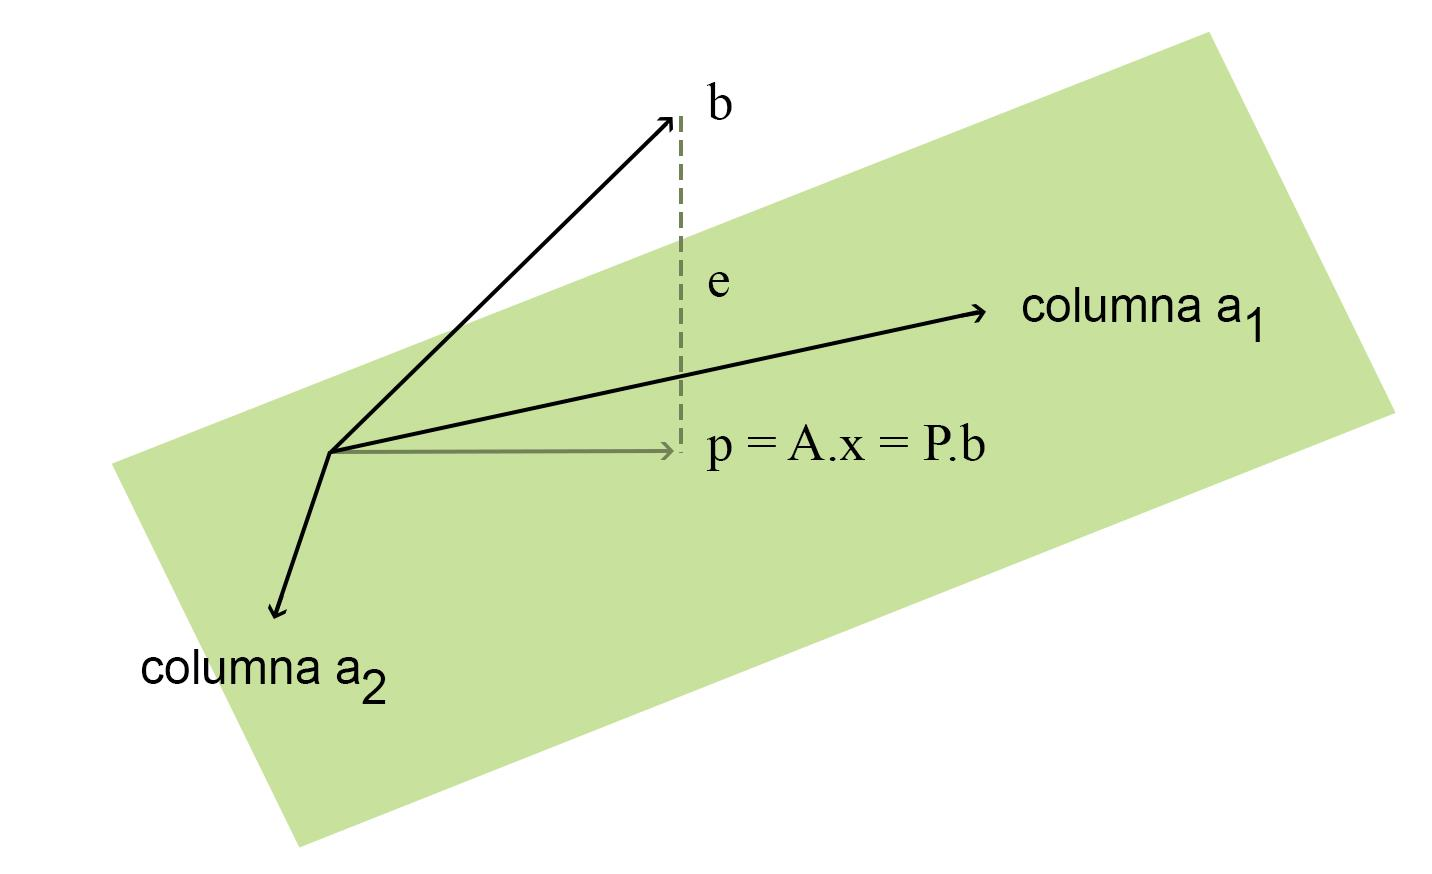
\includegraphics[width=0.80\textwidth]{Pictures/CUADM1.jpg}
    \caption{Proyección sobre el espacio columna.}
    \label{MINCUAD_1}
\end{figure}

\subsubsection{Un ejemplo de ajuste de datos  por  cuadrados mínimos}\index{Ajuste por cuadrados mínimos}

Supongamos realizamos un experimento en el que se espera que la salida $\textbf{b}$ sea una función lineal de la entrada $\textbf{t}$. Se buscará la recta $\textbf{b}= \alpha + \beta \textbf{t}$. Por ejemplo, si a diferentes tiempos medimos la distancia a un satélite en su recorrido a Marte. En este caso $\textbf{t}$ es el tiempo y $\textbf{b}$ la distancia y el satélite se moverá con una velocidad casi constante ($\textbf{b}=\textbf{b}_0 + v \textbf{t})$. 
¿Es posible calcular $\alpha$ y $\beta$ ? Si no hay errores experimentales dos mediciones determinan la recta $\textbf{b}= \alpha + \beta \textbf{t}$. Pero si hay error  se deberá promediar los experimentos y hallar la \textit{mejor} recta.
Al realizar $m$ mediciones, 

\begin{eqnarray*}
  \alpha + \beta t_1&=& b_1 \\
  \alpha + \beta t_2&=& b_2  \\
  \cdots  \\
  \alpha + \beta t_m&=& b_m
  \label{180}
\end{eqnarray*}

Se tendrá un sistema \textit{sobredeterminado}, con  $m$ ecuaciones y solo $2$ incógnitas. Si las mediciones tienen error, el sistema no tiene solución. En este caso la matriz $A$ tiene dos columnas  y $\textbf{x}=( \alpha, \beta)^T$:

\begin{eqnarray}
\left(\begin{array}{cc} 1 \quad t_1\\ 1  \quad t_2
\\  1  \quad t_3 \\ \cdots \\ 1  \quad t_m 
\end{array}\right) \left(\begin{array}{c} \alpha\\ \beta
\end{array}\right)= \left(\begin{array}{c} b_1\\ b_2
\\  b_3 \\ \cdots \\ b_m 
\end{array}\right)
\end{eqnarray}

o $A\textbf{x}=\textbf{b}$.
La mejor recta se tendrá con $\hat{\textbf{x}}= (\hat \alpha, \hat \beta)$ que minimizan 

$$E^2=\left\|A \textbf{x}-\textbf{b} \right\|^2= (b_1- \alpha- \beta t_1)^2 + (b_2- \alpha- \beta t_2)^2 +  \cdots (b_m- \alpha- \beta t_m)^2 $$.

El vector $\textbf{p}=A \hat{\textbf{x}}$ es el más cercano a $\textbf{b}$. De todas las rectas $\textbf{b}= \alpha + \beta \textbf{t}$ estamos eligiendo la que mejor ajusta los datos. 
%Ver figura (Strang  Figure 3.9). 
Los errores son las distancias verticales $\textbf{b}- \alpha - \beta t$ (no perpendiculares). Estas distancias verticales se elevan al cuadrado, se suman y se minimizan.



\bigskip


 
\begin{example}
    
\end{example}

Si se considera como ejemplo, que se tienen tres mediciones:
\noindent
$b_1=1$ en $t_1=-1$, $b_2=1$ en $t_2=1$  y $b_3=3$ en $t_3=2$ se tiene el sistema $Ax=b$

\begin{equation}
\left(\begin{array}{cc} 1 & -1  \\  1 &  1 \\  1 & 2 
\end{array}
 \right) \left(\begin{array}{c} \alpha \\  \beta 
\end{array}
 \right)=  \left(\begin{array}{c} 1    \\  1 \\  3
\end{array}
 \right)
 \label{190}
\end{equation}
 
 El sistema es incompatible porque los puntos no están sobre una misma recta. Se resuelve entonces, por cuadrados mínimos,
  $A^TA  \hat{\textbf{x}}=A^T\textbf{b}$
  
  \begin{equation}
\left(\begin{array}{cc} 3 & 2  \\  2 &  6 
\end{array}
 \right) \left(\begin{array}{c} \hat \alpha \\  \hat \beta 
\end{array}
 \right)=  \left(\begin{array}{c} 5    \\  6 
\end{array}
 \right)
 \label{200}
\end{equation}

\bigskip

La solución es $\hat \alpha= \frac{9}{7}$, $\hat \beta= \frac{4}{7}$ y la mejor recta es $ \frac{9}{7} + \frac{4}{7} t $.

\bigskip

Como se muestra  en la Figura \ref{MINCUAD_3}, el vector $\textbf{b}$ no es combinación lineal de las columnas $( 1,1,1)^T$ y $( -1,1,2)^T$. Con mínimos cuadrados se reemplaza $\textbf{b}$ que no está en la recta  por el vector $\textbf{p}=A \hat{\textbf{x}}$ que sí está, al no poder resolver $A\textbf{x}=\textbf{b}$, se resuelve $A \hat{\textbf{x}} = \textbf{p}$. El vector $\textbf{p}=( \frac{5}{7}, \frac{13}{7} ,\frac{17}{7}  )$  está en el espacio columna, es la proyección en ese subespacio. Restando $\textbf{p}$ de $\textbf{b}$, los errores son $\textbf{e}=\textbf{b}-\textbf{p}=( \frac{2}{7},  -\frac{6}{7}, \frac{4}{7} )$. Son los errores verticales en la Figura \ref{MINCUAD_2}. Ese vector $\textbf{e}$, como se muestra en la  Figura \ref{MINCUAD_3}, es ortogonal a las  columnas de $A$ (está en el espacio nulo de $A^T$).

\begin{figure}
    \centering
    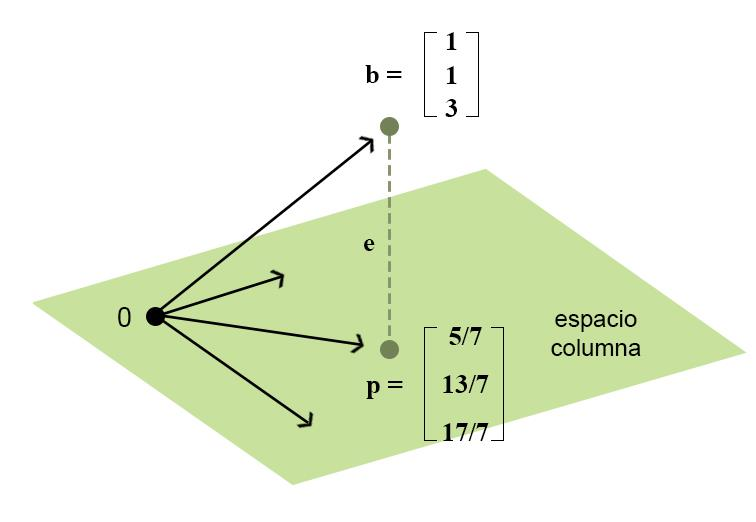
\includegraphics[width=0.80\textwidth]{Pictures/CUADM3.jpg}
    \caption{Proyección del vector $b$ en el espacio columna.}
    \label{MINCUAD_3}
\end{figure} 


\begin{figure}
    \centering
    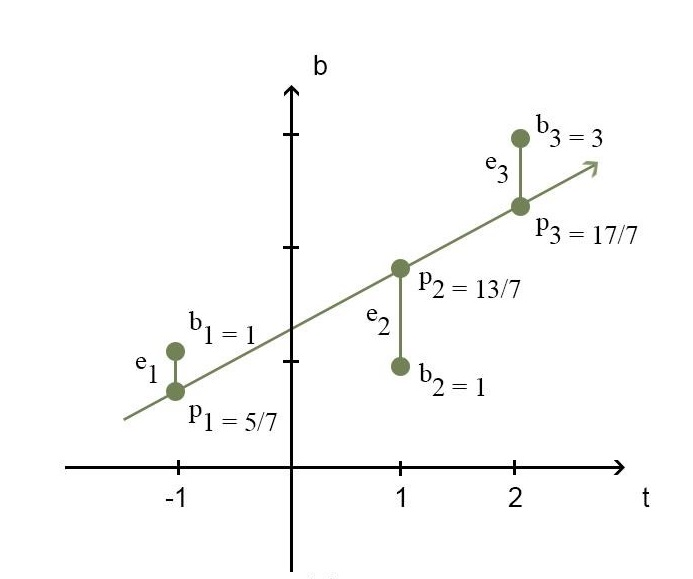
\includegraphics[width=0.75\textwidth]{Pictures/CUADM2.jpg}
    \caption{Recta que ajusta  por mínimos cuadrados los datos del ejemplo.}
    \label{MINCUAD_2}
\end{figure}
%\end{example}

Para el caso  de $m$ mediciones  $b_1, b_2,   \cdots, b_m$   en puntos  distintos $t_1, t_2,   \cdots, \\ t_m$, la recta  
$\alpha + \beta t$ que minimiza  $E^2$, surge de resolver el sistema lineal 

 \begin{equation}
A^TA\left(\begin{array}{c} \hat \alpha \\  \hat \beta 
\end{array}
 \right)= A^T b
 \label{210}
\end{equation}

o 

 \begin{equation}
\left(\begin{array}{cc} m & \sum_{i=1}^m t_i  \\  \sum_{i=1}^m t_i &  \sum_{i=1}^m t_i^2 
\end{array}
 \right) \left(\begin{array}{c} \hat \alpha \\  \hat \beta 
\end{array}
 \right)=  \left(\begin{array}{c} \sum_{i=1}^m b_i    \\ \sum_{i=1}^m t_i b_i
\end{array}
 \right)
 \label{220}
\end{equation}


 
  \bigskip
\begin{remark}  
Es importante notar que el método de cuadrados mínimos no está limitado a ajustar datos con una recta. En muchos casos interesan otros ajustes, con polinomios de grado más alto o con otras funciones como es el caso de ajuste  exponencial o el ajuste con senos y cosenos. Pueden conducir a problemas lineales o a problemas no lineales de cuadrados mínimos, siendo estos últimos  más complejos de abordar. 
\end{remark}


\begin{remark}
 El método por mínimos cuadrados fue inventado por Karl Friedrich Gauss, y lo usó para resolver un problema de astronomía. En 1801 el asteroide Ceres se había observado mucho más brillante durante más de un mes antes de desaparecer cuando se acercó al Sol. Con base en las observaciones disponibles, los astrónomos deseaban aproximar la órbita de Ceres para observarlo de nuevo cuando se alejara del sol. Gauss empleó los mínimos cuadrados e impactó a la comunidad científica al predecir la hora y el lugar correctos (unos 10 meses después) para localizar el asteroide.
 %\hfill$\blacktriangle$
\end{remark}


\index{Gauss, Karl Friedrich}
\begin{parchment}[Karl Friedrich Gauss (1777 - 1855)]{ Fue un matemático, astrónomo y físico alemán que contribuyó significativamente en muchos ámbitos, incluida la teoría de números, el análisis matemático, la geometría diferencial, la estadística, el álgebra, la geodesia, el magnetismo y la óptica. 

Gauss pronto fue reconocido como un niño prodigio, pese a provenir de una familia campesina de padres con poca cultura: su madre sabía leer, aunque no escribir; su padre sí, pero en cuanto a las matemáticas, no pasaba de la aritmética más elemental. De Carl Friedrich Gauss existen muchas anécdotas acerca de su asombrosa precocidad. Completó su magnum opus, Disquisitiones arithmeticae, a los veintiún años (1798), aunque la obra no se publicó hasta 1801. Constituye un trabajo fundamental como consolidación de la teoría de los números y ha moldeado esta área hasta los días presentes. \cite{gauss} }
\end{parchment} 


\section{Endomorfismos de espacios vectoriales con producto interno}\index{Endomorfismos}

Vamos a asociar ahora a cada endomorfismo  $f$ de un espacio vectorial $V$  de dimensión finita y con producto interno otra transformación lineal $f ^{*}$, $f ^{*}: V \rightarrow V  $.


\bigskip
\begin{definition}


Sea $V$ un espacio vectorial  con producto interno y sea $f$ una transformación lineal. Se llama \textit{adjunta} de $f$ y se anota  $f ^{*}$ a una transformación lineal $f ^{*}: V \rightarrow V  $ tal que 

 \begin{equation}
(f(\vec{v}),\vec{w})=(\vec{v},f ^{*}(\vec{w})) \qquad  \forall \vec{v},\vec{w}\in V
 \label{230}
\end{equation}
\end{definition}


\bigskip


\begin{example} 
\label{ejemplotadjunta}


Sea $f: \mathbb{C}^{2}\rightarrow  \mathbb{C}^{2}$ con el producto interno canónico, dada por 
$f(x,y)=((x+iy, 2x-(1+i)y)$


\bigskip


Se tiene que

\bigskip


% completar todos los pasos
$(f(x,y),(z,w))= ((x+iy, 2x-(1+i)y),(z,w) )= ((x,y), (z+2w,-iz+(-1+i)w))$ 

\bigskip
\noindent
de donde, $f ^{*}:  \mathbb{C}^{2}\rightarrow  \mathbb{C}^{2}  $ definida por $f ^{*}(z,w)=(z+2w, -iz+(-1+i)w)$ satisface 
$(f(x,y),(z,w))=((x,y),f ^{*}(z,w))$ para todo par de vectores $(x,y),(z,w)$ en $\mathbb{C}^{2}$.
\end{example}
\bigskip

  




El resultado que sigue prueba que  en espacios vectoriales   con producto interno de dimensión finita,   la transformación lineal adjunta existe y es única. 





\bigskip
\begin{theorem}

Sea $V$ un espacio vectorial de dimensión finita  con producto interno y sea $f$ una transformación lineal, $f: V \rightarrow V$. Entonces existe una única transformación lineal $f ^{*}: V \rightarrow V  $ tal que $$(f(\vec{v}),\vec{w})=(\vec{v},f ^{*}(\vec{w}))$$ 

\begin{proof}
Unicidad

Para ver la unicidad supongamos existen transformaciones lineales $g^{*}: V \rightarrow V$ y  $ h^{*}: V \rightarrow V $ tales que, para $\vec{w}$ fijo y para cada $\vec{v}$

$$ (f(\vec{v}), \vec{w})= (\vec{v},g(\vec{w}) )\qquad  (f(\vec{v}), \vec{w})= (\vec{v},h(\vec{w}))  $$
entonces 


$(\vec{v},g(\vec{w}))=(\vec{v},h(\vec{w}))$  o equivalentemente, $(\vec{v},g(\vec{w})-h(\vec{w}))=\vec{0}$, para todo $\vec{v} \in V$; tomando $ \vec{v}= g(\vec{w})-h(\vec{w})$, se tiene $(g(\vec{w})-h(\vec{w}),g(\vec{w})-h(\vec{w}))=0 $ y por la propiedad del producto escalar $g(\vec{w})-h(\vec{w})=0$, entonces $g(\vec{w})=h(\vec{w})$, para cada $\vec{w} \in V $, con lo cual $g$ y $h$ coinciden.

\bigskip

Existencia


Sea  $\left\{\vec{v}_1,\vec{v}_2, \cdots\vec{v}_n\right\}$ una base ortonormal de $V$. Si existe $f ^{*}: V \rightarrow V  $ con las condiciones del enunciado, debe cumplirse, para cada $\vec{w} \in V $


$$f ^{*}(\vec{w})= \sum_{i=1}^n (f ^{*}(\vec{w}), \vec{v}_i)\vec{v}_i$$

$$= \sum_{i=1}^n \overline{  ( \vec{v}_i,f ^{*}( w)})\vec{v}_i$$

$$ = \sum_{i=1}^n \overline{  (f(\vec{v}_i),\vec{w})}\vec{v}_i = \sum_{i=1}^n (\vec{w}, f(\vec{v}_i))\vec{v}_i  $$

Se define entonces, $f ^{*}: V \rightarrow V  $

\begin{equation}
  \label{adjunta}  
f ^{*}(\vec{w})= \sum_{i=1}^n (\vec{w},  f(\vec{v}_i))\vec{v}_i
\end{equation}

\bigskip

$f ^{*}$ es una transformación lineal


\begin{itemize}
     
    
    \item
    Usando la definición Ec.(\ref{adjunta} ),
    $$f ^{*}(\vec{w_1}+\vec{w_2} )=  \sum_{i=1}^n ( \vec{w_1}+\vec{w_2} ,  f(\vec{v}_i))\vec{v}_i $$
    
    $$=  \sum_{i=1}^n ( \vec{w_1} ,  f(\vec{v}_i)) + (\vec{w_2} ,  f(\vec{v}_i))\vec{v}_i $$
    
    $$=  \sum_{i=1}^n ( \vec{w_1} ,  f(\vec{v}_i))\vec{v}_i +  \sum_{i=1}^n (\vec{w_2} ,  f(\vec{v}_i))\vec{v}_i $$
    
    $$= f ^{*}(\vec{w_1} )+ f ^{*}(\vec{w_2} )$$
    
    \item
    
    
    Para $\lambda \in \mathbb{C} ($o$  \mathbb{R})$  $\vec{w} \in V$
    
    $$f ^{*}(\lambda \vec{w} )=  \sum_{i=1}^n ( \lambda \vec{w} ,  f(\vec{v}_i))\vec{v}_i $$
    
    $$ = \lambda \sum_{i=1}^n  (\vec{w} ,  f(\vec{v}_i))\vec{v}_i= \lambda f ^{*} (\vec{w})    $$
    
\end{itemize}

\bigskip


Veamos que para todo $ \vec{v},  \vec{w} \in V $ vale $(f(\vec{v}),\vec{w})=(\vec{v},f ^{*}(\vec{w}))$

\bigskip

Sean $ \vec{v},  \vec{w} \in V $. Se tiene que  $ \vec{v}= \sum_{i=1}^n ( \vec{v} ,  \vec{v}_i)\vec{v}_i $ y entonces, $ f(\vec{v})= \sum_{i=1}^n ( \vec{v} ,  \vec{v}_i)f(\vec{v}_i) $


$$ (f(\vec{v}),  \vec{w} )  = (\sum_{i=1}^n ( \vec{v} ,  \vec{v}_i)f(\vec{v}_i), \vec{w} )  $ $

$$  = \sum_{i=1}^n ( \vec{v} ,  \vec{v}_i)(f(\vec{v}_i), \vec{w} )   $$



Por otro lado 


$$( \vec{v},f ^{*}(\vec{w}))  =  (\sum_{i=1}^n ( \vec{v} ,  \vec{v}_i)\vec{v}_i),  \sum_{j=1}^n ( \vec{w} ,  f(\vec{v}_j))\vec{v}_j)     $$

$$  \sum_{i=1}^n ( \vec{v} ,  \vec{v}_i)(\vec{v}_i,  \sum_{j=1}^n ( \vec{w} ,  f(\vec{v}_j))\vec{v}_j)     $$

$$  \sum_{i=1}^n ( \vec{v} ,  \vec{v}_i)\sum_{j=1}^n  \overline{  ( \vec{w} ,  f(\vec{v}_j))  }( \vec{v}_i,  \vec{v}_j)$$  

$$\sum_{i=1}^n ( \vec{v} ,  \vec{v}_i) \overline{  ( \vec{w} ,  f(\vec{v}_i))  } = \sum_{i=1}^n ( \vec{v} ,  \vec{v}_i)  (  f(\vec{v}_i), \vec{w}  )   $$

\bigskip

Concluimos entonces que se cumple $(f(\vec{v}),\vec{w})=(\vec{v},f ^{*}(\vec{w}))$



\end{proof}
\end{theorem}




%COMPLETAR Unicidad. Existencia. 

%Se define $f ^{*}(\vec{w})= \sum^{n}_{i=1}(\vec{w},f(\vec{v}_i))\vec{v}_i$ , se prueba que es lineal y cumple lo pedido

\bigskip

\bigskip


A partir de la matriz de una transformación lineal $f: V \rightarrow V$ en una base ortonormal de $V$, puede obtenerse fácilmente la matriz de su adjunta en la misma base.


\bigskip


\begin{theorem}

Sea $V$ un espacio vectorial de dimensión finita  con producto interno y sea $f$ una transformación lineal, $f: V \rightarrow V$. Sea $B$ una base ortonormal de $V$. Entonces, la matriz que representa la transformación adjunta es la conjugada y transpuesta de la matriz de la transformación $f$, es decir,
\begin{equation}
(f^{*})_B= (( f )_B)^{*}
 \label{240}
\end{equation}



\bigskip

\begin{proof}

Supongamos que $B=\left\{\vec{v}_1,\vec{v}_2, \cdots\vec{v}_n\right\}$ es  una base ortonormal de $V$. Entonces para cada $1 \le i, j \le n$, 

$$((f^{*})_B)_{ij}= (f^{*}(\vec{v}_j), \vec{v}_i)$$
\noindent
como  en cada columna $j$ van las coordenadas de $f^{*}(\vec{v}_j$) en la base $B$,

$$=\overline{(\vec{v}_i, f^{*}(\vec{v}_j))}= \overline{(f(\vec{v}_i), \vec{v}_j)}= (\overline{( f )_B)})_{ji}= (( f )_B)^{*}_{ij} $$

\end{proof}

\end{theorem}

\bigskip

\bigskip

\begin{example}
En el caso de la transformación lineal adjunta del Ejemplo \ref{ejemplotadjunta}, si $B$ es la base canónica de $\mathbb{C}^{2}$, se tiene, de acuerdo a la proposición anterior, que la matriz que la representa es:

\bigskip

$(f)_B= \left(\begin{array}{cc}  1 & i  \\ 2 &  -1-i 
\end{array}
 \right)$  y   $ \qquad (f ^{*})_B= \left(\begin{array}{cc}  1 & 2  \\ -i &  -1+i 
\end{array}
 \right)$ \\
 
\noindent 
$(f ^{*})_B$ es la matriz transpuesta y conjugada de $(f)_B$.

  
\bigskip 


\end{example}



\bigskip

%Ver  propiedades del EH

Existe el caso particular de transformaciones lineales $f: V \rightarrow V$ cuya adjunta $f ^{*}$ coincide con $f$.

\bigskip

\begin{definition}\index{Transformación lineal autoadjunta} 

Sea $V$ un espacio vectorial  con producto interno y sea $f: V \rightarrow V$ una transformación lineal. Se dice que $f$ es \textit{autoadjunta}  si   $f= f ^{*}$ o sea, tal que


 \begin{equation}
(f(\vec{v}),\vec{w})=(\vec{v},f (\vec{w})) \qquad  \forall  ~ \vec{v}, \vec{w}\in V 
 \label{250}
\end{equation}
\end{definition}


\bigskip
\begin{definition}
 
Una matriz    $A \in \mathbb{R}^{n \times  n  }$   se dice \textit{simétrica} si $A _{ij}={A _{ji}}$    $\forall  1 \le i,j \le n$, o equivalentemente, si $A=A^T$. Una matriz  $A \in \mathbb{C}^{n \times  n  }$ se dice\textit{ hermitiana} si $A _{ij}=\overline {A _{ji}}$ $\forall  1 \le i,j \le n$, o equivalentemente, si $A=A^*$.  
\end{definition}
\bigskip

Si $A$ es la matriz de una transformación lineal $f$ en una base  ortonormal, sabemos que $A ^{*}$ es la matriz de la transformación adjunta en la misma base. Si $f$ es autoadjunta se tiene $A= A ^{*}$, por lo tanto la matriz de una transformación lineal autoadjunta es simétrica (hermítica).

%Ver propiedades de las autoadjuntas (p 385)









\bigskip

Si $f$ es autoadjunta, entonces, es una transformación lineal  diagonalizable. Más aún,  existe una base ortonormal de $V$ formada por autovectores de $f$ y todos sus autovalores son reales. 

\bigskip


\begin{theorem}

Sea $V$ un espacio vectorial  de dimensión finita con producto interno. Sea $f$ una transformación lineal autoadjunta. Entonces el polinomio característico de $f$ tiene todas sus raíces reales.

%\begin{proof}}
\end{theorem}
\bigskip

\begin{remark}
 Si $A \in \mathbb{C}^{n \times  n  }$ es una matriz hermitiana, entonces todas las raíces del polinomio característico de $A$ son reales.
 %\hfill$\blacktriangle$
\end{remark} 
 
\bigskip

El que sigue es un resultado importante sobre diagonalización de transformaciones lineales autoadjuntas.

\bigskip

\begin{theorem}
\label{diagreal}
Sea $V$ un espacio vectorial  de dimensión finita con producto interno. Sea $f: V \rightarrow V$ una transformación lineal autoadjunta. Entonces existe una base ortonormal $B$ de $V$  tal que la matriz $(f)_B$ es diagonal real.

\end{theorem}

\bigskip


\begin{remark}
 \begin{itemize}
     \item 
 Sea $A \in \mathbb{R}^{n \times  n  }$ es una matriz simétrica. Si se considera el producto interno canónico en $\mathbb{R}^{n}$, la transformación lineal $f_A: \mathbb{R}^{n}\rightarrow  \mathbb{R}^{n}$ definida por $f_A(\vec{x})=A\vec{x}$ es autoadjunta. Por la Proposición \ref{diagreal}  existe una base ortonormal $B$ de $\mathbb{R}^{n}$ tal que $(f_A )_B=D$, donde $D$ es una diagonal real. En este caso, si $E$ es la base canónica de $\mathbb{R}^{n}$, $(f_A )_E=A$,  $D= (P_{BE})^{-1}A(P_{BE})$, y  $(P_{BE})^{-1}=(P_{BE})^{t}$.
\item 
Análogamente, si    $A \in \mathbb{C}^{n \times  n  }$  es una matriz hermitiana. Si se considera $\mathbb{C}^{n}$ con   el producto interno canónico, la transformación lineal $f_A: \mathbb{C}^{n}\rightarrow  \mathbb{C}^{n}$,  definida por $f_A(\vec{x})=A\vec{x}$ es autoadjunta, y si $E$ es la base canónica de $\mathbb{C}^{n}$, $(f_A )_E=A$.
Por la proposición anterior  existe una base ortonormal $B$ de $\mathbb{C}^{n}$ tal que $(f_A )_B=D$, donde $D$ es una diagonal real. 
Entonces $ (P_{E,B})^{-1}A(P_{E,B})$, donde, por lo anterior $(P_{E,B})^{-1}=(P_{E,B})^{*}$.
% REVISAR SI $P_{BE}$   es la matriz de cambio de base de $B$ a $E$.
\end{itemize}
%\hfill$\blacktriangle$
\end{remark} 
\bigskip




Esto anterior nos lleva a la siguiente definición

\bigskip

\begin{definition}\index{Matriz ortogonal}\index{Matriz unitaria} 
\label{Matriz ortogonal}
Una matriz $O$ se dice \textit{ortogonal } si es invertible y $O^{-1}=O^{t}$.
Una matriz $U\in \mathbb{C}^{n \times  n  }$ se dice \textit{unitaria } si  es invertible y $U^{-1}=U^{*}$.
\end{definition} 


\begin{example}
Dada la matriz $A$,

\begin{equation}
A= \left(\begin{array}{cc} 1 & 1-i  \\ 1+i & 0
\end{array}
 \right), 
\end{equation}
se desea hallar una matriz unitaria $U$ tal que $U^{*}AU$  sea diagonal
\end{example}
Si en el programa Octave escribimos $[U,D]= eig(A)$
\noindent
nos devuelve las matrices $U$ y $D$ (con edición de $4$  dígitos):


\begin{equation}
U= \left(\begin{array}{cc} 0.4082-0.4082i & 0.5774-0.5774i  \\ -0.8165 & 0.5774
\end{array}
 \right), \qquad  D= \left(\begin{array}{cc} -1 & 0  \\ 0 & 2
\end{array}
 \right)
\end{equation}

\bigskip

Se verifican $U^{*}U=I$ y $U^{*}AU=D$


\bigskip

\bigskip

Resumiendo


\begin{enumerate}

\item  Sea   $A \in \mathbb{R}^{n \times  n  }$  una matriz simétrica. Entonces existe una matriz ortogonal  $O\in \mathbb{R}^{n \times  n  }$ tal que 
$O^{t}AO$ es diagonal.

%(En el Grossman está la demostración. Es el Teorema 3 del Capítulo 6, sección 4.)


\item Sea   $A \in \mathbb{C}^{n \times  n  }$ una matriz hermitiana. Entonces existe una matriz unitaria $C\in \mathbb{C}^{n \times  n  }$ tal que 
$C^{*}AC$ es diagonal real.


\end{enumerate}


\bigskip


\begin{remark}
    Toda transformación lineal autoadjunta en un espacio euclídeo de dimensión finita tiene sus autovalores reales
\end{remark}
\bigskip

%\begin{theom}
%(Diagonalización de matrices simétricas (hermíticas))
%La matriz de una transformación lineal autoadjunta puede ser reducida en una base ortonormal determinada %a una matriz diagonal.

%\end{theom}

\begin{example}

Se quiere diagonalizar ortogonalmente la matriz \index{Diagonalización}

\begin{equation}
A= \left(\begin{array}{cc} 1 & -2  \\ -2 & 3
\end{array}
 \right), \label{300}
\end{equation}

\bigskip


La ecuación característica de $A$ es $det(a- \lambda I)=  \left |\begin{array}{cc} 1-  \lambda & -2  \\ -2 & 3-\lambda  
\end{array}
 \right |= \lambda ^2 - 4 \lambda -1=0  $.
 
\bigskip
Tiene dos raíces, $\lambda_1= 2-\sqrt 5$  y  $\lambda_2= 2+\sqrt 5$


\bigskip


\noindent 
y los vectores propios correspondientes, son $ \vec{v}_1=  \left (\begin{array}{c} 2  \\ -1 + \sqrt 5  
\end{array}
 \right )$  y $ \vec{v}_2=  \left (\begin{array}{c} 1 - \sqrt 5   \\  2
\end{array}
 \right )$.
 
\bigskip

 %Notar que $\vec{v}_1. \vec{v}_2   =0$  (son ortogonales por teorema XX).
 
Para obtener vectores ortonormales los dividimos por su longitud, entonces,


\bigskip

$ \vec{u}_1= \frac{1}{\sqrt{10-2\sqrt 5}} \left (\begin{array}{c} 2  \\ -1 + \sqrt 5  
\end{array}
 \right )$ y  $ \vec{u}_2= \frac{1}{\sqrt{10-2\sqrt 5}} \left (\begin{array}{c} 1 - \sqrt 5   \\  2  
\end{array}
 \right )$

\begin{equation}
O= \frac{1}{\sqrt{10-2\sqrt 5}} \left(\begin{array}{cc} 2 & 1 - \sqrt 5 \\ -1 + \sqrt 5 & 2
\end{array}
 \right), \label{310}
\end{equation}

\bigskip

y $O^T A O =\left(\begin{array}{cc} 2-\sqrt 5 & 0  \\ 0 & 2+\sqrt 5
\end{array}
 \right)  $ 

\end{example}

\bigskip


\bigskip

\begin{example}



Sea 

\begin{equation}
A= \left(\begin{array}{cc} 2 & 3-3i  \\ 3+3i  & 5
\end{array}
 \right), \label{3000}
\end{equation}

\noindent
 una matriz hermitiana $\in \mathbb{C}^{2 \times 2}$.

 \bigskip
Es posible  diagonalizarla con la matriz unitaria 
 
\begin{equation}
U= \frac{1}{\sqrt{3}} \left(\begin{array}{cc} -1+i & 1 \\ 1 & 1+i
\end{array}
 \right), \label{320}
\end{equation}

\bigskip
\noindent
y se tiene que  $U^* A U =\left(\begin{array}{cc} -1 & 0  \\ 0 & 8
\end{array}
 \right)  $ 
es una matriz diagonal real.

\end{example}

\bigskip


\subsubsection{Transformaciones ortogonales}\index{Transformación ortogonal}
\label{Transf.Ortogonales}
Veremos ahora endomorfismos de un espacio vectorial con producto interno que preservan el producto interno y en particular, las distancias entre vectores.

\bigskip

\begin{theorem}

Sea $V$ un espacio euclídeo. Una transformación lineal $f$  se llama ortogonal si 
$(f(\vec{v}),f(\vec{w}))=(\vec{v},\vec{w})$ $~\forall \vec{v},\vec{w} \in V$. Es decir $f$ conserva el producto escalar.
\end{theorem}


\bigskip

\begin{theorem}
Toda transformación lineal $f$ en un espacio euclídeo  que conserve la longitud de los vectores  es una transformación ortogonal.

\begin{proof} 

$$\left\|f(\vec{v}+\vec{w})\right\|^{2}=   (f(\vec{v}+\vec{w}),f(\vec{v}+\vec{w})) $$

$$=\left\|f(\vec{v})\right\|^{2}  +2   (f(\vec{v}),f(\vec{w})) +  \left\|f(\vec{w})\right\|^{2} $$

\bigskip

\noindent
y, por otro lado, 

$$\left\|\vec{v}+\vec{w}   \right\|^{2} =   \left\|\vec{v}\right\|^{2} +2   (\vec{v},\vec{w}) +  \left\|\vec{w}\right\|^{2} $$

\bigskip

Como $f$ conserva la longitud de los vectores, $\left\|f(\vec{v}+\vec{w})\right\|=\left\|\vec{v}+\vec{w}\right\|$, $\left\|f(\vec{v})\right\|=\left\|\vec{v}\right\|$, $\left\|f(\vec{w})\right\|=\left\|\vec{w}\right\|$, entonces, igualando términos en las expresiones anteriores, se tiene que, 

\bigskip
$$(f(\vec{v}),f(\vec{w}))=(\vec{v},\vec{w}),$$

\noindent
y se  prueba que $f$ es ortogonal.

\end{proof} 
\end{theorem}

\bigskip

   \begin{example}
  
  $f=id_V$  es una transformación lineal ortogonal
\end{example} 

\bigskip


\begin{example} 
  
  
  Una rotación en $\mathbb{R}^{2}$ (con centro en el origen de coordenadas) es una transformación lineal ortogonal.
  
  Ya vimos en la Sección \ref{MatrizdeunaTL},  (Ec.(\ref{rot})) que la matriz de una  rotación en un ángulo $\theta$ en sentido antihorario, respecto de una base ortonormal es 
  
  \begin{equation}
R_{\theta}= \left(\begin{array}{cc} cos(\theta)   & -sen(\theta) \\ sen(\theta) & cos(\theta)
\end{array}
 \right), \label{400}
\end{equation}

\bigskip

Se verifica  que   $\forall \vec{v} \in \mathbb{R}^{2}  $,  $ \left\|R \vec{v}\right\|^{2} =  \left\|\vec{v}\right\|^{2}$
   \end{example} 
   
\bigskip
  
\begin{example}
  En $\mathbb{R}^{2}$ cualquier simetría con respecto a un subespacio vectorial unidimensional es una transformación lineal ortogonal.  
  
  
  En el caso de simetría respecto del eje $x$, en la base canónica, la matriz es 
  
  
  \begin{equation}
S= \left(\begin{array}{cc} 1   & 0\\ 0 & -1
\end{array}
 \right), \label{500}
\end{equation}



\end{example} 
  
\begin{remark}
\begin{itemize}
     \item 
     En $\mathbb{R}^{2}$ las únicas transformaciones ortogonales son las rotaciones y las simetrías, mientras que en
     $\mathbb{R}^{3}$ hay más  posibilidades de tener transformaciones lineales ortogonales que en $\mathbb{R}^{2}$.
\item
Para estudiar todas las posibles transformaciones lineales ortogonales se deben analizar los autovalores.
\item
Puede demostrarse que toda transformación lineal $f$ que transforma al menos una base ortonormal en una base ortonormal, es ortogonal.
\end{itemize}
\end{remark}

\bigskip


 \begin{example} 
En $\mathbb{R}^{3}$ la simetría con respecto a una recta, como se muestra  en la  Figura  \ref{SIM_3}.
La matriz de la transformación en la base $\{ \vec{u}_1, \vec{u}_2, \vec{u}_3  \}$ es 
%(ver Hernández figuras pág. 393).

\bigskip


$$\left(\begin{array}{ccc} 1  & 0  & 0  \\ 0 & -1 & 0  \\ 0 & 0 & -1
\end{array}
 \right)$$
\end{example} 

\begin{figure}
    \centering
    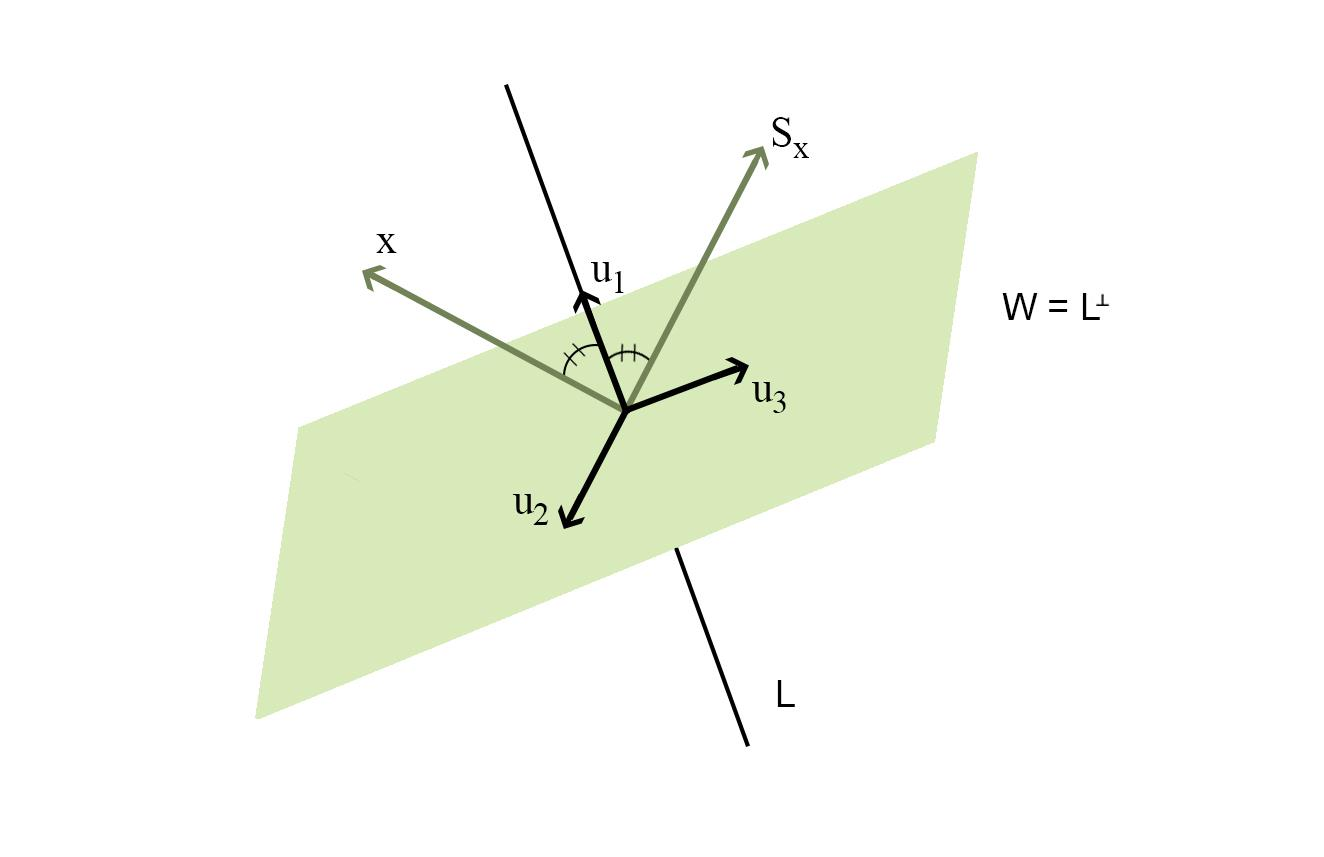
\includegraphics[width=0.80\textwidth]{Pictures/fig.32.jpg}
    \caption{Simetría con respecto a una recta.}
    \label{SIM_3}
\end{figure} 


\bigskip

 



\bigskip

\begin{theorem}
\label{det1ortog}

Los autovalores reales de una  transformación lineal ortogonal son iguales a $1$ o a $-1$.


\begin{proof}

Si $\lambda$ es un autovalor real de una transformación ortogonal, con autovector  $\vec{v}$, se tiene

$$(\vec{v},\vec{v})=(f(\vec{v}),f(\vec{v}))= ( \lambda \vec{v}, \lambda \vec{v})= \lambda ^2 (\vec{v},\vec{v})$$

Por lo tanto $ \lambda ^2 = 1$  y $ \lambda  = +- 1$. 

  \end{proof}
  \end{theorem}
\bigskip


\begin{remark} \index{Descomposición espectral de una matriz}
\begin{itemize}
    \item 

Una transformación lineal que cumple las  condiciones anteriores se dice unitaria  si $V$ es un $\mathbb{C}$ espacio vectorial y ortogonal si $V$ es un   $\mathbb{R}$ espacio vectorial.

\bigskip

$ f$ es unitaria (ortogonal) $\longleftrightarrow$  $(f)_B$ es unitaria (ortogonal) 

\bigskip

\item

Cuando A es simétrica y no demasiado grande, los algoritmos de computadora modernos que se usan  actualmente calculan con gran precisión vectores y valores propios.
Esos algoritmos aplican a $A$ una sucesión de transformaciones de semejanza en las
que intervienen matrices ortogonales.  El uso de matrices ortogonales evita que
los errores numéricos se acumulen durante el proceso. Cuando A es simétrica, la
sucesión de matrices ortogonales se combina para formar una matriz ortogonal cuyas
columnas son vectores propios de $A$.
Una matriz no simétrica no puede tener un conjunto completo de vectores propios
ortogonales, por lo que se necesitan técnicas no ortogonales para calcular los vectores
propios.


\bigskip

\item
Cuando una matriz $A$ tiene $n$ vectores propios ortogonales se llama \textit{descomposición espectral} de $A$ a la expresión

$$A= \lambda_1 \vec{u}_1^t \vec{u}_1 +\lambda_2 \vec{u}_2^t \vec{u}_2 + \cdots +\lambda_n \vec{u}_n^t \vec{u}_n.$$

La matriz $A$ queda dividida en partes determinadas por el espectro, y cada término es una matriz de rango $1$. Entre las aplicaciones de esta descomposición está la compresión de imágenes, que se realiza considerando  $k$ términos en lugar de $n$, con $k <n $, 
\end{itemize}
%\hfill$\blacktriangle$
\end{remark} 

\bigskip
%
%\end{document}

\newpage

%\begin{figure}
    %\centering
    %
\includegraphics[width=0.60\textwidth]{Pictures/prodint.png}    
    %\label{TLfig12}
%\end{figure}



\section{Actividades propuestas}
\begin{answers}

De acuerdo con la segunda ley de Kepler, un cometa debería tener una órbita elíptica,\index{Orbita de un cometa} parábolica o hiperbólica (despreciando las atracciones gravitacionales de los planetas). En convenientes coordenadas polares, la posición (r,$\vartheta$) de un cometa satisface una ecuación de la forma:

$$r=\beta+ e(r.\cos(\vartheta))$$

\noindent
donde $\beta$ es una constante y $e$ es la excentricidad de la órbita (con $0\leq e \le 1$ para una elipse,
e=1 para una parábola, y $e\ge 1$ para una hipérbola).
Suponga que los siguientes datos corresponden a las observaciones de un cometa recién descubierto. 

\bigskip

\begin{table*}[ht]
	\centering
					\begin{tabular}{lccccc}
\hline\hline
$\vartheta$&0.88&1.10&1.42&1.77&2.14\\
\hline
r &3.00&2.30&1.65&1.25&1.01\\
		\end{tabular}
\end{table*}
Determine el tipo de órbita e indique dónde estará el cometa cuando $\vartheta$=4.6 radianes.

\bigskip

\end{answers}

\bigskip

 \subsection{Ejercicios}
 
 \bigskip
%\subsubsection{Espacios Vectoriales con Producto Interno.}
 
 
\begin{exercise}
\item
Sea $\mathbb{E}$ un espacio euclídeo, si $\vec{x},\vec{y}$ y $\vec{z}$ son vectores de $\mathbb{E}$, desarrolle la siguiente expresión: ($\vec{x} +\vec{z}, \vec{x}-\vec{z}+\vec{y}$)
\end{exercise}
\begin{exercise}
\item

Calcule la distancia entre los vectores $\vec{u}=(2,i,1-i)$ y $\vec{v}=(-i,0,4i)$ en  $\mathbb{C}^3$ con el producto interno canónico. 
\end{exercise}


\begin{exercise}
\item

Pruebe que las siguientes  funciones definen productos internos sobre los espacios vectoriales considerados


a)   $  (\cdot,\cdot)$: $ C\left[0,1\right] \times C\left[0,1\right]  \rightarrow  \mathbb{R}, (f(x),g(x))= \int_0^1f(x)g(x)dx$.

b)   $   (\cdot,\cdot)$:  $K^{n \times n}  \times K^{n \times n}\rightarrow K$,(A,B)=$tr(A.B^*)$, con $K=\mathbb{R}$ y $K=\mathbb{C}$ ($B^*$ es la matriz traspuesta conjugada de B). 
\end{exercise}

\begin{exercise} 
\item

Determine para qué valores de $\alpha \in \mathbb{R} $:
\[
\phi((x_1,x_2),(y_1,y_2))=x_1y_1-x_1y_2-x_2y_1+\alpha x_2y_2
\]
es un producto interno en $\mathbb{R}^2$.
\end{exercise}
\begin{exercise}
\item

Sean $\vec{u}_1=(-2,-1,1),\vec{u}_2=(0,-1,0)$ y $\vec{u}_3=(1,-1,0)$ tres vectores linealmente independientes de $\mathbb{R}^3$. Si definimos el producto
escalar en $\mathbb{R}^3$ afirmando que $\{\vec{u}_1,\vec{u}_2,\vec{u}_3\}$ es una base ortonormal. ¿Cuál sería la expresión analítica de este producto escalar
en la base canónica de $\mathbb{R}^3$?

\end{exercise}


\bigskip

%\subsubsection{Matrices ortogonales y complemento ortogonal}

\vspace{0.25cm}

\begin{exercise}
\item
Demuestre que $Q$  $\in \mathbb{R}^{2 \times  2  }$ es una matriz de rotación puesto que $Q$ es ortogonal y además su determinante vale $1$.
$Q=\left(\begin{array}{cc}\cos(\phi) & -\sin(\phi) \\ \sin(\phi)& \cos(\phi)
\end{array}
 \right)$
\end{exercise}
\begin{exercise}

\bigskip

\item
En $P^{(2)}_{\mathbb{R}}\left[x\right]$ se define el producto escalar:
$\phi(p(x),q(x))= \int_{-1}^1p(x)q(x)dx$

\noindent Pruebe que el conjunto $\left\{1,x, \frac{1}{3}(3x^2 -1)\right\}$ es ortogonal.
\end{exercise}

\begin{exercise}
\item

Dada la matriz simétrica 
$A=\left(\begin{array}{cc}1 & -2 \\-2 & 1
\end{array}
 \right)$
 construya una matriz ortonormal $T$ tal que $(T^{-1}AT)$ sea una matriz diagonal. Verifique
 también que  $T^{-1}=T^{t}$ y que el determinante de $T$ es igual a 1. Obtenga asimismo la matriz
 diagonal $(T^{-1}AT)$.
\end{exercise}

%\newpage

\begin{exercise}
\item

Halle una base ortogonal de $\mathbb{R}^3$ -con el producto interno canónico- que contenga al vector $\vec{u}=(1,-1,2)$.
\end{exercise}
\begin{exercise}
\item
Sea 
\[A=\left(\begin{array}{ccc}1 & -2 & 0   \\ -2& 2 & -2
\\ 0  & -2 & 3                         
\end{array}
 \right)
\]

a) Halle una base ortonormal de autovectores de $A$.

b) Halle una matriz $P$ ortogonal tal que $P^tAP$ sea diagonal.
\end{exercise}
\begin{exercise}
\item


Sea $B=\{(1,0,1),(2,0,1),(1,1,0)\}$ una base de $\mathbb{R}^3$. Considere el producto interno canónico y utilice Gram-Schmidt para hallar a partir de $B$ una base $B^{\prime}$ que sea ortonormal. Calcule las coordenadas de $\vec{v}=(2,-1,3)$ en la base $B\prime$. Utilice sus resultados para encontrar la factorización $A=QR$.  Puede chequear sus resultados utilizando el diguiente programa Python:

\bigskip

\begin{lstlisting}[language = python, numbers = none, escapechar = !,
    basicstyle = \ttfamily\bfseries, linewidth = 1\linewidth] 
import numpy as np
# Definimos la matriz
A = np.array([[4, 3, 1],
              [2, 1, 3],
              [1, 1, 1]])
# Realizamos la descomposición QR
Q, R = np.linalg.qr(A)
# Imprimimos las matrices Q y R
print("Matriz Q:")
print(Q)
print("Matriz R:")
print(R)
\end{lstlisting}

\end{exercise}
\begin{exercise}
\item
Demuestre que S=$\left\{\vec{u}_1,\vec{u}_2,\vec{u}_3\right\}$ es un conjunto ortogonal donde

\bigskip


$\vec{u}_1=\left(\begin{array}{c} 3   \\ 1\\ 1                           
\end{array}
 \right) ,\vec{u}_2=\left(\begin{array}{c} -1   \\ 2\\ 1                           
\end{array}
 \right), \vec{u}_3=\left(\begin{array}{c} -\frac{1}{2}  \\ -2\\ \frac{7}{2}                       
\end{array} \right), \vec{y}=\left(\begin{array}{c} 6   \\ 1\\ -8                           
\end{array} \right)$


\bigskip

\noindent Exprese el vector $\vec{y}$
como combinación lineal del conjunto S. Recuerde las coordenadas se calculan cómo $c_j= (\frac{\vec{y}.\vec{u_j}}{\vec{u_j}\vec{u_j}})$ con $j=1,2,3$ por ser ortogonal.

\bigskip

\end{exercise}
\begin{exercise}
\item
Calcule la distancia de un punto $\vec{y}$ en $\mathbb{R}^3$ a un subespacio W generado por $\left\{\vec{u}_1,\vec{u}_2\right\}$ sabiendo que el punto más cercano se calcula como $\left\|\vec{y}-\hat{y}\right\|$, donde $\hat{y}=proy_w \vec{y}$.

\bigskip

$\vec{y}=\left(\begin{array}{c} -1   \\ -5\\ 10                           
\end{array}
 \right),\ vec{u}_1=\left(\begin{array}{c} 5   \\ -2\\ -1                           
\end{array}
 \right),\ vec{u}_2=\left(\begin{array}{c} 1   \\ 2\\ -1                          
\end{array} \right)$
\end{exercise}

\begin{exercise}
\item

Halle el complemento ortogonal para el siguiente subespacios de $V$:

$V=\mathbb{R}^3$, $S_1=\{(x_1,x_2,x_3)\in \mathbb{R}^3,  2x_1-x_2=0\} $ para el producto interno canónico.

\end{exercise}


\begin{exercise}
\item

Demuestre que el conjunto $S=  \{   cos nx,sen mx \}_{n,m \in  \mathbb{N}}$  es linealmente independiente en $C([0, 2 \pi])$.
Sugerencia: observar que 



$$\int_0^{2\pi}  (cos^2 nx )dx \neq 0, \quad   \int_0^{2\pi}  (sen^2 mx )dx \neq 0, \quad  n,m \in  \mathbb{N} $$ 

y 

$$\int_0^{2\pi}  (cos nx )(cos mx) dx =  \quad   \int_0^{2\pi}  (cos nx )(sen mx)) dx = 

=\quad  \int_0^{2\pi}  (sen nx )(sen mx) dx=0 $

\bigskip

si $n \neq m, n, m  \in  \mathbb{N} $ 

\bigskip

\end{exercise}


\newpage
 
%\subsubsection{Operador Adjunto. Operador Unitario }

\begin{exercise}
\item

Halle $T^*$ para cada una de las transformaciones lineales siguientes:

a) $T:\mathbb{R}^2 \rightarrow \mathbb{R}^2$, $T((x_1,x_2))=(3x_1+x_2,-x_1+x_2)$.\\

b) $T:\mathbb{R}^3 \rightarrow \mathbb{R}^3$, tal que $\left[T \right]_B=\left(\begin{array}{ccc}1 & 0 & 1   \\ 2& 0 & -1
\\ 0  & 1 & 0                         
\end{array}
 \right)$, 
 
 donde $B=\{(1,2,-1),(1,0,0),(0,1,1)\}$.

 \bigskip
 
 
%c)  $T:P^{(2)}_{\mathbb{R}}[x] \rightarrow P^{(2)}_{\mathbb{R}}[x]$, $T(p)=p'$, $(f,g)= \int_0^1f(x)g(x)dx$.

\end{exercise}

\begin{exercise}
\item
Determine si los siguientes endomorfismos definidos sobre $\mathbb{R}^3$ son autoadjuntos:

a) $T((x,y,z))=(x+y,x,-z)$

b) $S((x,y,z))=(-2x+2z,y,2x)$
\end{exercise}

\begin{exercise}
\item 

Encuentre en cada caso una matriz $O \in \mathbb{R}^{n \times n}$  ortogonal tal que $O.A.O^t$ sea diagonal

\bigskip

a) $A=\left(\begin{array}{cc}1 &  3   \\ 3 & -1
                       
\end{array}
 \right)$

\bigskip

b) $A=\left(\begin{array}{ccc}5 & 0 & -2   \\ 0 & 7 & -2
\\ -2  & -2 & 6                         
\end{array}
 \right)$

 
 

\end{exercise}

\newpage

\begin{exercise}
\item 


Dada 
$A=\left(\begin{array}{cccc}4 &1 & i & 0    \\ 1 & 3 & 2i
&0 \\ -i  & -2i & 3  & i \\0 & 1 &-i & 2                         
\end{array}
 \right)$

 \bigskip
 

\noindent encuentre una matriz $U \in \mathbb{C}^{n \times n}$  ortogonal tal que $U.A.U^*$ sea diagonal.
\end{exercise}
\begin{exercise}
\item

Halle la matriz en la base canónica de las siguientes transformaciones ortogonales

a)  $T:\mathbb{R}^2 \rightarrow \mathbb{R}^2$, rotación de un ángulo de $\frac {\pi}{4}$.


b)  $T:\mathbb{R}^2 \rightarrow \mathbb{R}^2$, simetría respecto de la recta $x_1=x_2$.

\end{exercise}

\bigskip

% \subsection{Ejercicios teóricos}\\
 
 \bigskip

\begin{exercise} 
\item

Sea $V$ un espacio vectorial y sea $(\cdot,\cdot)$ un producto interno sobre $V$. Pruebe

a) $( \Vec{x}, \Vec{y}+\Vec{z})= ( \Vec{x}, \Vec{y} ) +( \Vec{x}, \Vec{z} )$


b) $( \Vec{x}, c\Vec{y} )= \overline c ( \Vec{x}, \Vec{y} )$

c) $( \Vec{x}, \Vec{y})=  (\Vec{x},\Vec{z} )  \quad  \forall \Vec{x} \in V  \Rightarrow \Vec{y}=\Vec{z}$
\end{exercise}

\begin{exercise}
\item 


Sea $V$ un espacio vectorial con producto interno   $(\cdot,\cdot)$. Pruebe que $\left|(\Vec{x}, \Vec{y} )\right| =\left\|\Vec{x}\right\|\left\|\Vec{y}\right\|$ sí y sólo sí $\{\Vec{x},\Vec{y}\}$ es un conjunto linealmente dependiente.
\end{exercise}
\begin{exercise}
\item
Pruebe que dos vectores $\vec{x}$ e $\vec{y}$  son ortogonales, si 

$\left\|\vec{x}+\vec{y}\right\|^{2}=\left\|\vec{x}\right\|^{2}+\left\|\vec{y}\right\|^{2}$
\end{exercise}
%\newpage

\begin{exercise}
\item

Sea  $V$ un espacio vectorial sobre $K$ de dimensión finita con producto interno  $(\cdot,\cdot)$. Sea $T \in L(V)$ biyectivo. Considerar la aplicación    $(\cdot,\cdot)_{T}: V \times V \rightarrow  K$, $(\vec{x}, \vec{y})_{T} =( T(\vec{x}) ,T(\vec{y}))$, $~\forall \vec{x}, \vec{y} \in V$

\noindent Pruebe que $(\cdot,\cdot)_{T}$ también es un producto interno sobre $V$.
\end{exercise}
\begin{exercise}
\item

Sea $A \in   \mathbb{R}^{2 \times 2}$. Sea $\phi: \mathbb{R}^2 \times \mathbb{R}^2 \rightarrow \mathbb{R}$ definida por $\phi(x,y)=y.A.x^t$. Pruebe  que $\phi$ es un producto interno sobre $\mathbb{R}^2$ si y sólo sí $A=A^t$, $\~A_{11} \geq 0$ y $Det(A) \geq 0$.

\end{exercise}

\begin{exercise}
\item


Sea $V$ un $\mathbb{C}$-espacio vectorial con producto interno  $(\cdot,\cdot)$ y sea $T \in L(V)$ sobre $\mathbb{C}$. Pruebe que si $\lambda$ es autovalor  de $T$,  entonces  $\overline \lambda$ es un autovalor de $T^*$.
\end{exercise}

\begin{exercise}
\item


Sea $V$ un $\mathbb{C}$-espacio vectorial con producto interno  $(\cdot,\cdot)$ y sea $T \in L(V)$ sobre $\mathbb{C}$ autoadjunto. Pruebe que:


a)  si $\lambda$ es autovalor  de $T$,  entonces  $\lambda  \in \mathbb{R}$.

b) Si $v_i$ es autovector asociado al autovalor $\lambda_i$ de $T$ (para $i=1$,$2$) y $\lambda_1 \neq \lambda_2$, entonces
$(\vec{v_1}, \Vec{v_2})=0$.

\end{exercise}
\begin{exercise}
\item

Sea V un espacio vectorial de dimensión finita con producto interno y sean $S$ y $T$ $\in L(V)$. Si $k \in K$, pruebe:

a) $(S+T)^*=S^*+T^*$

b) $(kT)^*=\overline k T^*$

c)  $(ST)^*=T^*S^*$
\end{exercise}




\bigskip
 

 \subsection{Autoevaluación}
 \label{Auto4}
 \bigskip



\subsubsection{Verdadero o Falso.}


\bigskip

\begin{enumerate}
  

\item
El subespacio imagen de una transformación lineal es ortogonal a su núcleo.

\item
El vector cero es ortogonal a todo vector en $\mathbb{R}^n$.

\item
Sean W un plano a travéz del origen en $\mathbb{R}^3$ y L la recta que pasa por el origen y es perpendicular a W. Entonces $L^{\bot}=W$ y $W^{\bot}=L$.
\item
$T(\vec{x})=(\frac{\vec{x}.\vec{v}}{\vec{v}\vec{v}}).\vec{v}$ es una transformación de proyección.
\item
Una matriz cuadrada U tal que $U^{-1}=U^t$ se denomina ortogonal.
\item
Si $U$ es ortonormal tanto las filas como las columnas de U son ortonormales.
\item
En la factorización $QR$ el hecho de que R sea invertible es consecuencia directa de que las columnas de A sean linealmente independientes.
\item
Si $\left\{\vec{v}_1,\vec{v}_2,\vec{v}_3\right\}$ es una base ortogonal para W, entonces la multiplicación de $\vec{v}_3$ por un escalar, da una nueva base ortogonal  $\left\{\vec{v}_1,\vec{v}_2,3\vec{v}_3\right\}$
\item
Si $A=QR$, donde $Q$ tiene columnas ortonormales, entonces R=$Q^t A$.
\item
Si $\vec{x}$ no esta en un subespacio W, entonces $\vec{x}-proy_w \vec{x}$ no es cero.
\item
Un espacio vectorial con un producto escalar se dice que es un espacio vectorial euclídeo.
\item
Si $Q$ es ortogonal se cumple que la norma de $\vec{x}$ es igual a la norma de $Q\vec{x}$.
\item
Todo conjunto ortogonal de un espacio euclídeo es linealmente dependiente. 
\item
El determinante de una matriz ortogonal es $1$ ó $-1$.
\item
El producto de dos matrices ortogonales es la matriz identidad. 
\item
El rango de $A$ es $n$ si y sólo si $A^t=A$ es invertible.
\item
Descomponer un vector $\vec{y}$ en una suma de proyecciones ortogonales sobre espacios unidimensionales es la esencia del proceso de Gram-Smith.
\item
dim V = dim W + dim $W^{\bot}$.
\item
$d(\vec{u},-\vec{v})^2$= $\left\|\vec{u}+\vec{v}\right\|^2= \left\|\vec{u}\right\|^2 + \left\|\vec{v}\right\|^2 + 2\vec{u}\vec{v}$.



\end{enumerate}

\bigskip

%\begin{lstlisting}[language = python, numbers = none, escapechar = !,
%    basicstyle = \ttfamily\bfseries, linewidth = 1\linewidth] 
%import numpy as np
%a = np.random.randn(9, 6)
%q, r = np.linalg.qr(a)
%print(a)
%np.allclose(a, np.dot(q, r))  # a does equal qr
%r2 = np.linalg.qr(a, mode='r')
%np.allclose(r, r2)  # mode='r' returns the same r as mode='full'
%a = np.random.normal(size=(3, 2, 2)) # Stack of 2 x 2 matrices as input
%q, r = np.linalg.qr(a)
%print('matriz q')
%q.shape
%r.shape
%c=np.allclose(a, np.matmul(q, r))
%\end{lstlisting}

\bigskip